%===============================================================================
% LaTeX sjabloon voor de bachelorproef toegepaste informatica aan HOGENT
% Meer info op https://github.com/HoGentTIN/latex-hogent-report
%===============================================================================

\documentclass[dutch,dit,thesis]{hogentreport}

% Beperk (waarschuwingen voor verwaarloosbare) over- en underfull-instanties
\hfuzz=5.0pt
\hbadness=10000
\setlength{\emergencystretch}{3em}

% Maak gebruik van listings

\usepackage{listings}
\usepackage{xcolor}

% Maak gebruik van .svg-bestanden

% \usepackage{svg}

\definecolor{codegreen}{rgb}{0,0.6,0}
\definecolor{codegray}{rgb}{0.5,0.5,0.5}
\definecolor{codepurple}{rgb}{0.58,0,0.82}
\definecolor{backcolour}{rgb}{0.95,0.95,0.92}

\lstdefinestyle{mystyle}{
    backgroundcolor=\color{backcolour},   
    commentstyle=\color{codegreen},
    keywordstyle=\color{magenta},
    numberstyle=\tiny\color{codegray},
    stringstyle=\color{codepurple},
    basicstyle=\ttfamily\footnotesize,
    breakatwhitespace=false,         
    breaklines=true,                 
    captionpos=b,                    
    keepspaces=true,                 
    numbers=left,                    
    numbersep=5pt,                  
    showspaces=false,                
    showstringspaces=false,
    showtabs=false,                  
    tabsize=2
}

\lstset{style=mystyle}

% TODO:
% - If necessary, replace the option `dit`' with your own department!
%   Valid entries are dbo, dbt, dgz, dit, dlo, dog, dsa, soa
% - If you write your thesis in English (remark: only possible after getting
%   explicit approval!), remove the option "dutch," or replace with "english".

\usepackage{lipsum} % For blind text, can be removed after adding actual content

%% Pictures to include in the text can be put in the graphics/ folder
\graphicspath{{../graphics/}}

%% For source code highlighting, requires pygments to be installed
%% Compile with the -shell-escape flag!
%% \usepackage[chapter]{minted}
%% If you compile with the make_thesis.{bat,sh} script, use the following
%% import instead:
\usepackage[chapter,outputdir=../output]{minted}
\usemintedstyle{solarized-light}

%% Formatting for minted environments.
\setminted{%
    autogobble,
    frame=lines,
    breaklines,
    linenos,
    tabsize=4
}

%% Ensure the list of listings is in the table of contents
\renewcommand\listoflistingscaption{%
    \IfLanguageName{dutch}{Lijst van codefragmenten}{List of listings}
}
\renewcommand\listingscaption{%
    \IfLanguageName{dutch}{Codefragment}{Listing}
}
\renewcommand*\listoflistings{%
    \cleardoublepage\phantomsection\addcontentsline{toc}{chapter}{\listoflistingscaption}%
    \listof{listing}{\listoflistingscaption}%
}

% Other packages not already included can be imported here

%%---------- Document metadata -------------------------------------------------
% TODO: Replace this with your own information
\author{Lucas Ludueña-Segre}
\supervisor{Dhr. A. Veldeman}
\cosupervisor{Dhr. Y. Rousseaux}
\title[Onderzoek \& proof-of-concept]%
    {Omzetten van UML-diagrammen\\(PlantUML) naar ``configuration\\management''-code (Ansible)}
\academicyear{\advance\year by -1 \the\year--\advance\year by 1 \the\year}
\examperiod{2}
\degreesought{\IfLanguageName{dutch}{Professionele bachelor in de toegepaste informatica}{Bachelor of applied computer science}}
\partialthesis{true} %% To display 'in partial fulfilment'
%\institution{Internshipcompany BVBA.}

%% Add global exceptions to the hyphenation here
\hyphenation{back-slash}

%% The bibliography (style and settings are  found in hogentthesis.cls)
\addbibresource{bachproef.bib}            %% Bibliography file
\addbibresource{../voorstel/voorstel.bib} %% Bibliography research proposal
\defbibheading{bibempty}{}

%% Prevent empty pages for right-handed chapter starts in twoside mode
\renewcommand{\cleardoublepage}{\clearpage}

\renewcommand{\arraystretch}{1.2}

%% Content starts here.
\begin{document}

%---------- Front matter -------------------------------------------------------

\frontmatter

\hypersetup{pageanchor=false} %% Disable page numbering references
%% Render a Dutch outer title page if the main language is English
\IfLanguageName{english}{%
    %% If necessary, information can be changed here
    \degreesought{Professionele Bachelor toegepaste informatica}%
    \begin{otherlanguage}{dutch}%
       \maketitle%
    \end{otherlanguage}%
}{}

%% Generates title page content
\maketitle
\hypersetup{pageanchor=true}

%%=============================================================================
%% Voorwoord
%%=============================================================================

\chapter*{\IfLanguageName{dutch}{Woord vooraf}{Preface}}%
\label{ch:voorwoord}

%% TODO:
%% Het voorwoord is het enige deel van de bachelorproef waar je vanuit je
%% eigen standpunt (``ik-vorm'') mag schrijven. Je kan hier bv. motiveren
%% waarom jij het onderwerp wil bespreken.
%% Vergeet ook niet te bedanken wie je geholpen/gesteund/... heeft

% \lipsum[1-2]

De kern van deze bachelorproef is ontstaan uit een idee dat eerst werd voorgesteld door Thomas Clauwaert -- docent voor (onder andere) het \emph{OLOD} (opleidingsonderdeel) \emph{Cybersecurity Advanced} binnen de opleiding \emph{Toegepaste Informatica} op \emph{HOGENT}. Zijn initiële vraag -- hoe een infrastructuur, gevisualiseerd in een graaf, geautomatiseerd kan worden opgezet door \emph{configuration management} tools -- heb ik vanuit een nieuwe lens bekeken en uitgewerkt tot de uiteindelijke tool die in dit werk wordt beschreven.

Dit proces was bijzonder uitdagend, en het pad naar het einde was allesbehalve rechtlijnig. Het bouwen van de brug tussen punt A (de diagrammen) en punt B (de effectieve omgeving) heeft veel tijd, energie en doorzettingsvermogen van mij gevraagd. Wat me heeft doen doorzetten, is het keer op keer oplossen van het ene probleem na het andere -- tot ik uiteindelijk een resultaat bereikt heb waar ik oprecht trots op ben.
Ik ben er sterk van overtuigd dat ik mij nog zal blijven bezighouden met dit project (ook na mijn studies), in de hoop dat dit de drempel zal verlagen voor docenten en studenten om kwalitatieve IT-omgevingen sneller en efficiënter te kunnen opzetten.

Graag wil ik hier de kans nemen om een aantal mensen bedanken.

Allereerst mijn promotor, \textbf{Alexander Veldeman}, voor zijn begeleiding, gerichte feedback en steun doorheen beide semesters, alsook voor de oprechte interesse die hij heeft getoond in mijn idee en de tool die eruit is ontstaan.

Vervolgens mijn co-promotor, \textbf{Yoeri Rousseaux} van District09 (mijn stagebedrijf), die mij op technisch vlak meermaals heeft geholpen om het noorden terug te vinden dankzij zijn lange werkervaring in de IT-sector.

Uiteraard gaat een bijzonder dankwoord uit naar \textbf{Thomas Clauwaert}, voor het initiële idee dat aan de basis ligt van deze bachelorproef, en voor zijn boeiende lessen die ik heb kunnen volgen tijdens \emph{Cybersecurity \& Virtualisation} en \emph{Cybersecurity Advanced}.

Daarnaast wil ik \textbf{Bert Van Vreckem} bedanken voor zijn bijdrage aan de opleiding en, bij uitbreiding, aan deze bachelorproef. Zonder zijn \emph{Ansible}-rollen en \emph{Ansible Skeleton} zou deze tool niet de vorm hebben kunnen aannemen die deze vandaag heeft.

Ten slotte wil ik ook de andere docenten van de opleiding \emph{Toegepaste Informatica} bedanken voor de kennis, ervaring en passie die zij me hebben meegegeven tijdens mijn jaren op \emph{HOGENT}.

\begin{flushright}
    \emph{Lucas Ludueña-Segre, Gent, mei 2026}
\end{flushright}
%%=============================================================================
%% Samenvatting
%%=============================================================================

% TODO: De "abstract" of samenvatting is een kernachtige (~ 1 blz. voor een
% thesis) synthese van het document.
%
% Een goede abstract biedt een kernachtig antwoord op volgende vragen:
%
% 1. Waarover gaat de bachelorproef?
% 2. Waarom heb je er over geschreven?
% 3. Hoe heb je het onderzoek uitgevoerd?
% 4. Wat waren de resultaten? Wat blijkt uit je onderzoek?
% 5. Wat betekenen je resultaten? Wat is de relevantie voor het werkveld?
%
% Daarom bestaat een abstract uit volgende componenten:
%
% - inleiding + kaderen thema
% - probleemstelling
% - (centrale) onderzoeksvraag
% - onderzoeksdoelstelling
% - methodologie
% - resultaten (beperk tot de belangrijkste, relevant voor de onderzoeksvraag)
% - conclusies, aanbevelingen, beperkingen
%
% LET OP! Een samenvatting is GEEN voorwoord!

%%---------- Nederlandse samenvatting -----------------------------------------
%
% TODO: Als je je bachelorproef in het Engels schrijft, moet je eerst een
% Nederlandse samenvatting invoegen. Haal daarvoor onderstaande code uit
% commentaar.
% Wie zijn bachelorproef in het Nederlands schrijft, kan dit negeren, de inhoud
% wordt niet in het document ingevoegd.

% \IfLanguageName{english}{%
% \selectlanguage{dutch}
% \chapter*{Samenvatting}
% % \lipsum[1-4]
% \selectlanguage{english}
% }{}

%%---------- Samenvatting -----------------------------------------------------
% De samenvatting in de hoofdtaal van het document

\chapter*{\IfLanguageName{dutch}{Samenvatting}{Abstract}}

% \lipsum[1-4]

% Binnen de opleiding \emph{Toegepaste Informatica} op HOGENT worden studenten geconfronteerd met infrastructuurlabo's waarbij een gegeven netwerkontwerp manueel moet worden omgezet naar een werkende, geconfigureerde omgeving. Dit proces is tijdrovend en foutgevoelig, en vereist een grondige kennis van zowel de gebruikte diagramnotatie als de onderliggende configuratiebeheerstools. Deze bachelorproef onderzoekt in welke mate dit omzettingsproces geautomatiseerd kan worden.

Op HOGENT, binnen de opleiding \emph{Toegepaste Informatica} en meerbepaald het keuzetraject ``System \& Network Administrator'', worden er OLODs (opleidingsonderdelen) gegeven die aan de hand van labo's bijdragen aan het leren van serverinfrastructuren beheren. Deze infrastructuren worden geïmplementeerd aan de hand van netwerk- en implementatiediagrammen, ontworpen met UML-modeling software.
De probleemstelling voor deze bachelorproef vertrekt vanuit het foutgevoelige en tijdrovende proces waarbij (complexe) UML-diagrammen eerst geïnterpreteerd en daarna manueel vertaald worden naar een configureerbare infrastructuur.

De hoofdonderzoeksvraag luidt: Hoe kan men een gegeven netwerk- en implementatiediagram (in tekstuele vorm via bijvoorbeeld PlantUML\footnote{\url{https://plantuml.com/}}) van een infrastructuur met minimale menselijke interventie omzetten tot een overeenkomende, gebruiksklare `\emph{configuration management}'-ondersteunde (bijvoorbeeld met Ansible) omgeving?

Om deze vraag te beantwoorden werd een proof-of-concept converter ontwikkeld genaamd \emph{PlantUML2Ansible}. Het script neemt PlantUML-diagrammen als invoer -- meer bepaald een netwerk- en implementatiediagram -- en produceert op basis daarvan een omgeving die volledig wordt ondersteund door Vagrant en Ansible.
De converter ondersteunt twee gebruiksscenario's: een ``volledige modus'' die zowel `\emph{Infrastructure-as-Code}'- als `\emph{configuration management}'-uitvoer produceert, en een ``enkel-IaC-modus'' die zich enkel beperkt tot een Vagrant-omgeving.

De methodologie bestaat uit de volgende fasen: de literatuurstudie, het ontwerp en de implementatie van de testomgeving, de ontwikkeling van de converter, en de opstelling en uitvoering van testcases op basis van bestaande labo-omgevingen uit de opleidingsonderdelen \emph{Infrastructure Automation} en \emph{Cybersecurity Advanced}.

De resultaten tonen aan dat het technisch haalbaar is om, op basis van PlantUML-bronbestanden, volledige en functionele omgevingen te genereren zonder manuele tussenkomst. De labo-omgeving van \emph{Cybersecurity Advanced} werd succesvol gereproduceerd via de ``enkel-IaC-modus'', en die van \emph{Infrastructure Automation} via de ``volledige modus'' (zonder routering).

De proof-of-concept kent een aantal beperkingen: de volledige modus ondersteunt slechts één netwerk, enkel \emph{AlmaLinux} 9 wordt ondersteund als gastbesturingssysteem, en de diagrammen moeten vooraf voldoen aan een welomschreven deelverzameling van de PlantUML-syntax. 
Deze beperkingen vormen echter potentiëel voor toekomstige uitbreidingen, alsook alternatieve IaC-backends en compatibiliteit met IPv6.

De voornaamste meerwaarde van deze oplossing situeert zich in de educatieve context waarvoor ze ontworpen is. Docenten kunnen via deze tool hun labo-ontwerpen sneller effectief implementeren, terwijl studenten zo gemakkelijker en al experimenterend nieuwe infrastructuur-gerelateerde ideeën vorm kunnen geven.

%---------- Inhoud, lijst figuren, ... -----------------------------------------

\tableofcontents

% In a list of figures, the complete caption will be included. To prevent this,
% ALWAYS add a short description in the caption!
%
%  \caption[short description]{elaborate description}
%
% If you do, only the short description will be used in the list of figures

\listoffigures

% If you included tables and/or source code listings, uncomment the appropriate
% lines.
\listoftables

\listoflistings

% Als je een lijst van afkortingen of termen wil toevoegen, dan hoort die
% hier thuis. Gebruik bijvoorbeeld de ``glossaries'' package.
% https://www.overleaf.com/learn/latex/Glossaries

%---------- Kern ---------------------------------------------------------------

\mainmatter{}

% De eerste hoofdstukken van een bachelorproef zijn meestal een inleiding op
% het onderwerp, literatuurstudie en verantwoording methodologie.
% Aarzel niet om een meer beschrijvende titel aan deze hoofdstukken te geven of
% om bijvoorbeeld de inleiding en/of stand van zaken over meerdere hoofdstukken
% te verspreiden!

%%=============================================================================
%% Inleiding
%%=============================================================================

\chapter{\IfLanguageName{dutch}{Inleiding}{Introduction}}%
\label{ch:inleiding}

% De inleiding moet de lezer net genoeg informatie verschaffen om het onderwerp te begrijpen en in te zien waarom de onderzoeksvraag de moeite waard is om te onderzoeken. In de inleiding ga je literatuurverwijzingen beperken, zodat de tekst vlot leesbaar blijft. Je kan de inleiding verder onderverdelen in secties als dit de tekst verduidelijkt. Zaken die aan bod kunnen komen in de inleiding~\autocite{Pollefliet2011}:

% \begin{itemize}
%   \item context, achtergrond
%   \item afbakenen van het onderwerp
%   \item verantwoording van het onderwerp, methodologie
%   \item probleemstelling
%   \item onderzoeksdoelstelling
%   \item onderzoeksvraag
%   \item \ldots
% \end{itemize}

\section{Context, achtergrond}%
\label{sec:inl_context}

Binnen de opleiding \emph{Toegepaste Informatica} op \emph{HOGENT} hebben de meeste \emph{OLODs} (opleidingsonderdelen) gelinkt aan het keuzeprofiel ``\emph{IT infrastructure engineer}'' de opzet om het beheer van (virtuele) serveromgevingen aan te leren. Bij het opzetten van dit soort infrastructuur is helderheid over elke stap van het proces en communicatie met elke (al dan niet technisch ingestelde) stakeholder cruciaal.
Om deze duidelijkheid te waarborgen, wordt er binnen de opleiding (meerbepaald tijdens de analyse-\emph{OLODs}) ook aangeleerd om te werken met \emph{UML}-modeling software zoals \emph{Visual Paradigm}\footnote{\url{https://www.visual-paradigm.com/}} en \emph{draw.io}\footnote{\url{https://www.drawio.com/}}. Deze software wordt gebruikt om diagrammen te ontwerpen zoals Activity Diagrams, System Sequence Diagrams, domeinmodellen en BPMN-diagrammen. Deze diagrammen zijn hoofdzakelijk gericht op softwareontwikkeling.

Met deze software kan men ook netwerk- en implementatiediagrammen ontwerpen, die de specificaties, software-elementen (databanken, webservers, firewalls, \ldots) en verbanden tussen verschillende servers in een bepaalde infrastructuur verduidelijken. Deze servers worden op basis van deze diagrammen daarna respectievelijk opgezet via \emph{Infrastructure-as-Code}-tools (zoals \emph{Terraform}\footnote{\url{https://developer.hashicorp.com/terraform}}, \emph{OpenTofu}\footnote{\url{https://opentofu.org/}}, \emph{Vagrant}\footnote{\url{https://developer.hashicorp.com/vagrant}}, \ldots) en geconfigureerd met ``\emph{configuration management}''-tools (\emph{Ansible}\footnote{\url{https://docs.ansible.com/}}, \emph{Puppet}\footnote{\url{https://www.puppet.com/}}, \emph{Chef}\footnote{\url{https://www.chef.io/}}, \ldots). De \emph{HOGENT}-\emph{OLODs} ``\emph{DevOps Project: Operations}'', ``\emph{Cybersecurity Advanced}'' en meerbepaald ``\emph{Infrastructure Automation}'' introduceren ook het gebruik van \emph{Ansible}, één van de leidende ``\emph{configuration management}''-tools.

\section{\IfLanguageName{dutch}{Probleemstelling}{Problem Statement}}%
\label{sec:inl_probleemstelling}

% Uit je probleemstelling moet duidelijk zijn dat je onderzoek een meerwaarde heeft voor een concrete doelgroep. De doelgroep moet goed gedefinieerd en afgelijnd zijn. Doelgroepen als ``bedrijven,'' ``KMO's'', systeembeheerders, enz.~zijn nog te vaag. Als je een lijstje kan maken van de personen/organisaties die een meerwaarde zullen vinden in deze bachelorproef (dit is eigenlijk je steekproefkader), dan is dat een indicatie dat de doelgroep goed gedefinieerd is. Dit kan een enkel bedrijf zijn of zelfs één persoon (je co-promotor/opdrachtgever).

Het huidige proces waarbij (complexe) netwerk- en implementatiediagrammen worden geïnterpreteerd en manueel worden omgezet tot een ``\emph{configuration management}''-ondersteunde serveromgeving kan, volgens \textcite{Nicacio2020}, tijdrovend en vatbaar voor ambiguïteit en foute interpretaties zijn.

Bij implementatiediagrammen kan er onder meer onduidelijkheid onstaan bij (de versies van) software-packages, hun afhankelijkheden/dependencies, de firewall-regels voor elke server en hoe dit het bereik buiten het lokale netwerk beïnvloedt.
Voor netwerkdiagrammen kan dit bijvoorbeeld gaan over hardwarespecificaties van de servers, (de versies van) hun besturingssystemen en de declaratie van de \emph{DNS} server(s).

\section{\IfLanguageName{dutch}{Hoofdonderzoeksvraag}{Research question}}%
\label{sec:inl_hoofdonderzoeksvraag}

% Wees zo concreet mogelijk bij het formuleren van je onderzoeksvraag. Een onderzoeksvraag is trouwens iets waar nog niemand op dit moment een antwoord heeft (voor zover je kan nagaan). Het opzoeken van bestaande informatie (bv. ``welke tools bestaan er voor deze toepassing?'') is dus geen onderzoeksvraag. Je kan de onderzoeksvraag verder specifiëren in deelvragen. Bv.~als je onderzoek gaat over performantiemetingen, dan 

De hoofdonderzoeksvraag voor deze bachelorproef luidt als volgt:

Hoe kan men een gegeven netwerk- en implementatiediagram (in tekstuele vorm via bijvoorbeeld \emph{PlantUML}\footnote{\url{https://plantuml.com/}}) van een infrastructuur met minimale menselijke interventie omzetten tot een overeenkomende, gebruiksklare ``\emph{configuration management}''-ondersteunde (bijvoorbeeld met \emph{Ansible}) omgeving?

Voor deze omgeving wordt ervan uit gegaan dat de eenheden (bare-metal servers, virtuele machines, containers, \ldots) alvorens uitgerold zijn via een \emph{Infrastructure-as-Code}-tool en dat ze enkel nog achteraf geconfigureerd moeten worden via een ``\emph{configuration management}''-tool.

% TODO: Eventueel andere deelvragen vinden of bestaande vervangen, afhankelijk van de inhoud van de komende hoofdstukken

\section{Deelvragen over het probleemdomein}%
\label{sec:inl_deelvragen_probleemdomein}

\begin{itemize}
  \item Wat zijn de doeleinden (business- of technisch-gericht) van \emph{UML}?
  \item Welke infrastructuur-gerelateerde informatie kan een netwerk- en implementatiediagram \emph{niet} weergeven (dat een \emph{Infrastructure-as-Code}- en/of ``\emph{configuration management}''-tool wel kan)?
  \item Welke stappen zijn er tussen het ontwerp van \emph{UML}-diagrammen en de eerste opstelling van een ``\emph{configuration management}''-ondersteunde omgeving?
\end{itemize}

\section{Deelvragen over het oplossingsdomein}%
\label{sec:inl_deelvragen_oplossingsdomein}

\begin{itemize}
  \item Naast \emph{PlantUML} en \emph{MermaidJS}, met welke andere talen kan men \emph{UML}-diagrammen ontwerpen?
  \item Buiten \emph{Ansible}, \emph{Puppet} en \emph{Chef}, wat zijn andere ``\emph{configuration management}''-tools die voor dit soort doeleinden geschikt zijn?
  \item Aangezien er al tools bestaan om \emph{UML}-diagrammen te genereren op basis van ``\emph{configuration management}''-ondersteunde omgevingen, zoals één van \textcite{teramako2023}, welke meerwaarde zou deze oplossing (die in de omgekeerde richting werkt) kunnen bieden?
  \item Is het mogelijk om deze oplossing te ontwikkelen aan de hand van ``reverse engineering'' van de bovenstaande tools?
\end{itemize}

\section{\IfLanguageName{dutch}{Onderzoeksdoelstelling}{Research objective}}%
\label{sec:inl_onderzoeksdoelstelling}

% Wat is het beoogde resultaat van je bachelorproef? Wat zijn de criteria voor succes? Beschrijf die zo concreet mogelijk. Gaat het bv.\ om een proof-of-concept, een prototype, een verslag met aanbevelingen, een vergelijkende studie, enz.

De doelstelling van deze bachelorproef is om een proof-of-concept te ontwikkelen voor een converter (of omzetter) van \emph{PlantUML}-diagrammen naar \emph{Ansible}-code. \emph{PlantUML} en \emph{Ansible} zijn de twee tools die op dit moment voor ogen staan, maar er zullen tijdens het onderzoek ook alternatieven gezocht en geëvalueerd worden.

Deze oplossing zal een meerwaarde bieden voor educatieve doeleinden binnen de opleiding \emph{Toegepaste Informatica}. Neem als voorbeeld een \emph{OLOD} zoals ``\emph{Cybersecurity Advanced}'' -- een vak waarin studenten leren om de beveiliging van netwerken te versterken aan de hand van virtuele labo's. De tech-industrie evolueert snel en de labo's die voor dit \emph{OLOD} ontworpen zijn, zullen daardoor ook snel verouderen.

Aangezien met deze oplossing de drempel tussen de ontwerp- en implementatiefase verkleint, zouden docenten sneller nieuwe (virtuele) labo-omgevingen kunnen ontwerpen, met (in theorie) onmiddelijk beschikbare ``\emph{configuration management}''-code om deze meteen te configureren. Voor studenten kan dit ook een kans bieden om potentiële infrastructuur-gerelateerde experimenten tijdens hun studies sneller effectief vorm te geven.

\section{\IfLanguageName{dutch}{Opzet van deze bachelorproef}{Structure of this bachelor thesis}}%
\label{sec:inl_opzet-bachelorproef}

% Het is gebruikelijk aan het einde van de inleiding een overzicht te
% geven van de opbouw van de rest van de tekst. Deze sectie bevat al een aanzet
% die je kan aanvullen/aanpassen in functie van je eigen tekst.

De rest van deze bachelorproef is als volgt opgebouwd:

In Hoofdstuk~\ref{ch:literatuurstudie} (\nameref{ch:literatuurstudie}) wordt een overzicht gegeven van de stand van zaken binnen het onderzoeksdomein, op basis van een literatuurstudie.

In Hoofdstuk~\ref{ch:methodologie} (\nameref{ch:methodologie}) worden de verschillende fases van dit onderzoek toegelicht, alsook de gebruikte onderzoekstechnieken om antwoorden te kunnen formuleren op de hoofdonderzoeksvraag en deelvragen.

% Vul hier aan voor je eigen hoofstukken, één of twee zinnen per hoofdstuk

In Hoofdstuk~\ref{ch:manuele_testomgeving} (\nameref{ch:manuele_testomgeving}) wordt het ontwerp en de implementatie van de manuele testomgeving voor de proof-of-concept beschreven. Dit bevat een evaluatie van bestaande tools in de betrokken vakgebieden (\emph{UML} en \emph{configuration management}), alsook het ontwerp van de verwachte invoer en uitvoer voor de converter.

In Hoofdstuk~\ref{ch:poc} (\nameref{ch:poc}) wordt toegelicht hoe de proof-of-concept, in de vorm van een converter voor \emph{PlantUML} naar \emph{Ansible} (\emph{PlantUML2Ansible}), is ontwikkeld.

In Hoofdstuk~\ref{ch:testcases} (\nameref{ch:testcases}) wordt de definitie van de verschillende testcases, waar de converter op wordt getoetst, beschreven. De resultaten van deze testen worden ook in dit hoofdstuk toegelicht.

In Hoofdstuk~\ref{ch:conclusie_discussie} (\nameref{ch:conclusie_discussie}), ten slotte, wordt de conclusie gegeven en een antwoord geformuleerd op de onderzoeksvragen. Daarnaast wordt in de discussie ook een aanzet gegeven voor toekomstig onderzoek binnen dit domein.
%%=============================================================================
%% Literatuurstudie
%%=============================================================================

\chapter{\IfLanguageName{dutch}{Literatuurstudie}{State of the art}}%
\label{ch:literatuurstudie}

% Tip: Begin elk hoofdstuk met een paragraaf inleiding die beschrijft hoe
% dit hoofdstuk past binnen het geheel van de bachelorproef. Geef in het
% bijzonder aan wat de link is met het vorige en volgende hoofdstuk.

% Pas na deze inleidende paragraaf komt de eerste sectiehoofding.

% Dit hoofdstuk bevat je literatuurstudie. De inhoud gaat verder op de inleiding, maar zal het onderwerp van de bachelorproef *diepgaand* uitspitten. De bedoeling is dat de lezer na lezing van dit hoofdstuk helemaal op de hoogte is van de huidige stand van zaken (state-of-the-art) in het onderzoeksdomein. Iemand die niet vertrouwd is met het onderwerp, weet nu voldoende om de rest van het verhaal te kunnen volgen, zonder dat die er nog andere informatie moet over opzoeken \autocite{Pollefliet2011}.

% Je verwijst bij elke bewering die je doet, vakterm die je introduceert, enz.\ naar je bronnen. In \LaTeX{} kan dat met het commando \texttt{$\backslash${textcite\{\}}} of \texttt{$\backslash${autocite\{\}}}. Als argument van het commando geef je de ``sleutel'' van een ``record'' in een bibliografische databank in het Bib\LaTeX{}-formaat (een tekstbestand). Als je expliciet naar de auteur verwijst in de zin (narratieve referentie), gebruik je \texttt{$\backslash${}textcite\{\}}. Soms is de auteursnaam niet expliciet een onderdeel van de zin, dan gebruik je \texttt{$\backslash${}autocite\{\}} (referentie tussen haakjes). Dit gebruik je bv.~bij een citaat, of om in het bijschrift van een overgenomen afbeelding, broncode, tabel, enz. te verwijzen naar de bron. In de volgende paragraaf een voorbeeld van elk.

% \textcite{Knuth1998} schreef een van de standaardwerken over sorteer- en zoekalgoritmen. Experten zijn het erover eens dat cloud computing een interessante opportuniteit vormen, zowel voor gebruikers als voor dienstverleners op vlak van informatietechnologie~\autocite{Creeger2009}.

% Let er ook op: het \texttt{cite}-commando voor de punt, dus binnen de zin. Je verwijst meteen naar een bron in de eerste zin die erop gebaseerd is, dus niet pas op het einde van een paragraaf.

% \begin{figure}
%   \centering
%   
\includegraphics[width=0.8\textwidth]{grail.jpg}
%   \caption[Voorbeeld figuur.]{\label{fig:grail}Voorbeeld van invoegen van een figuur. Zorg altijd voor een uitgebreid bijschrift dat de figuur volledig beschrijft zonder in de tekst te moeten gaan zoeken. Vergeet ook je bronvermelding niet!}
% \end{figure}

% \begin{listing}
%   \begin{minted}{python}
%     import pandas as pd
%     import seaborn as sns

%     penguins = sns.load_dataset('penguins')
%     sns.relplot(data=penguins, x="flipper_length_mm", y="bill_length_mm", hue="species")
%   \end{minted}
%   \caption[Voorbeeld codefragment]{Voorbeeld van het invoegen van een codefragment.}
% \end{listing}

% \lipsum[7-20]

% \begin{table}
%   \centering
%   \begin{tabular}{lcr}
%     \toprule
%     \textbf{Kolom 1} & \textbf{Kolom 2} & \textbf{Kolom 3} \\
%     $\alpha$         & $\beta$          & $\gamma$         \\
%     \midrule
%     A                & 10.230           & a                \\
%     B                & 45.678           & b                \\
%     C                & 99.987           & c                \\
%     \bottomrule
%   \end{tabular}
%   \caption[Voorbeeld tabel]{\label{tab:example}Voorbeeld van een tabel.}
% \end{table}

Dit hoofdstuk biedt de stand van zaken en theoretische onderbouwing voor de vakgebieden die aan bod komen tijdens de ontwikkeling van de \emph{Proof of Concept}.

\section{\emph{Unified Modeling Language} (\emph{UML})}%
\label{sec:uml}

``\emph{Unified Modeling Language}'', of afgekort \emph{UML}, is een taal/framework die binnen de softwareontwikkeling-discipline geaccepteerd is als de standaard voor het weergeven van object-georiënteerde modellen. \emph{UML} wordt hoofdzakelijk gebruikt in de industrie-, business- en IT-sector, met als doel om de ontwerp- en implementatiefase te ondersteunen met verscheidene diagrammen. Deze kunnen door zowel business als technische stakeholders geïnterpreteerd worden voor hun respectievelijke doeleinden. \autocite{Koc2021}

Binnen de opleiding \emph{Toegepaste Informatica} worden er momenteel voornamelijk twee \emph{UML}-modeling programma's gebruikt en aangeraden; \emph{Visual Paradigm} en \emph{draw.io}. Dit zijn twee tools die (onder andere) werden geëvalueerd tijdens een vergelijkende studie van \textcite{Lu2023}, waarin \emph{Visual Paradigm} 122/165 (tweede plaats) en \emph{draw.io} 114/165 (achtste plaats, maar nog boven het gemiddelde) scoorden. Deze score is gebaseerd op hoe goed deze tools de verschillende diagramtypen ondersteunen, alsook of deze al dan niet bepaalde functionaliteiten bevatten zoals bestandsexportering en collaboratie.

Deze \emph{UML}-modeling programma's zijn \emph{GUI}-gebaseerd, en werken dus eerder met een drag-en-drop systeem. Er bestaan echter ook alternatieve tools zoals \emph{PlantUML} en \emph{MermaidJS}\footnote{\url{https://mermaid.js.org}}, die niet doorgaans vanuit de opleiding worden aangereikt. Deze maken, in tegenstelling tot \emph{Visual Paradigm} en \emph{draw.io}, gebruik van declaratieve talen waarmee men \emph{UML}-diagrammen kan ontwerpen via menselijk leesbare tekstbestanden, wat ook gemakkelijker te onderhouden is met versiebeheertools zoals \emph{Git}\footnote{\url{https://git-scm.com/}} \autocite{Romeo2025}.
Deze tools zijn ook open-source; de broncode van deze software is voor iedereen beschikbaar, wat voor studenten en docenten binnen de opleiding bijzonder interessant is.

\subsection{Diagrammen}%

Volgens \textcite{Padmanabhan2012} worden binnen \emph{UML} er veertien diagramtypen onderscheiden volgens de volgende overkoepelende categoriëen; \emph{Structure}, \emph{Behavior} en \emph{Interaction Diagrams}. Hier zijn een aantal van deze diagramtypen die het meest binnen de opleiding \emph{Toegepaste Informatica} toegelicht worden:

\begin{description}
  \item \textbf{\emph{Use Case Diagram}}: Beschrijft welke actoren (gebruikers, externe systemen) met een gegeven systeem interageren en welke functionaliteit zij gebruiken. Dit diagram is nuttig om de scope en de rollen binnen dit systeem te verduidelijken.
  \item \textbf{\emph{Class Diagram}}: Toont de klassen in een systeem met hun attributen, methoden en relaties (associaties, erfenis, compositie). Deze diagrammen zijn typisch op softwarecode gericht.
  \item \textbf{\emph{Deployment Diagram} (of implementatiediagram)}: Richt zich op de (al dan niet virtuele) nodes (servers, containers, netwerkapparatuur) en de daarop gedeployde artefacten (\emph{packages}, \emph{services}). Dit diagram sluit nauw aan bij een netwerkdiagram zoals die in DevOps-scenario's voorkomen.
  \item \textbf{\emph{Activity Diagram}}: Beschrijft de flow van controle en gegevens in een proces. Dit kan toegepast worden op een deployment pipeline of een provisioning workflow in een \emph{Infrastructure-as-Code}-context.
  \item \textbf{\emph{Sequence Diagram}}: Legt vast welke berichten in welke volgorde uitgewisseld worden tussen objecten of componenten, bijvoorbeeld tussen een webserver en een databank tijdens een typische request-flow.
\end{description}

\subsection{\emph{PlantUML}}%

\emph{PlantUML} is een open-source tool waarmee \emph{UML}- en aanverwante diagrammen gegenereerd kunnen worden op basis van een declaratief en menselijk leesbaar tekstformaat \autocite{PlantUML2026}.

De tool ondersteunt een brede waaier aan diagramtypen, waaronder vele \emph{UML}-diagrammen (\emph{Class Diagrams}, \emph{Deployment Diagrams}, \emph{Activity Diagrams}, \ldots), maar dus ook notaties die niet strikt genomen onder \emph{UML} vallen zoals netwerkdiagrammen, mindmaps en \emph{GANTT}-schemas \autocite{PlantUML2025}.

\emph{PlantUML} kan op verschillende manieren gebruikt worden; via de online webinterface\footnote{https://www.plantuml.com/plantuml}, een lokale installatie of een \emph{Docker}-container. Er worden ook verscheidene integraties aangeboden zoals plugins voor gangbare \emph{IDE}'s (\emph{Visual Studio Code}, \emph{IntelliJ IDEA} en \emph{Eclipse}) en documentatie- en wiki-tools (\emph{Confluence} en \emph{Markdown}).

Aangezien de diagramdefinities gewone tekstbestanden zijn (met ``\texttt{.puml}'' als bestandsextensie), lenen ze zich goed tot versiebeheer met \emph{Git}. \autocite{PlantUML2025a}

Het volgende codefragment stelt een voorbeeld van een implementatiediagram voor, met vijf nodes en hun bijhorende connecties.

\begin{codeblock}
  \begin{lstlisting}[language=plantuml]
@startuml

node node1
node node2
node node3
node node4
node node5
node1 -- node2 : label1
node1 .. node3 : label2
node1 ~~ node4 : label3
node1 == node5

@enduml
\end{lstlisting}
  \caption[Voorbeeld implementatiediagram in tekstformaat (\emph{PlantUML})]{Tekstformaat voor een voorbeeld van een implementatiediagram, uitgedrukt in \emph{PlantUML} \autocite{PlantUML2025}.}
  \label{code:depdiag_vb_puml}
\end{codeblock}

\emph{PlantUML} verwerkt vervolgens deze tekst en genereert op basis hiervan de volgende afbeelding.

\begin{figure}[H]
  \centering
  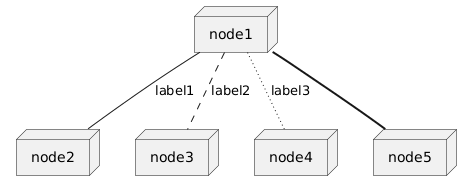
\includegraphics[width=0.5\textwidth]{../graphics/depdiag_vb_puml.png}
  \caption[Voorbeeld implementatiediagram in afbeeldingsformaat (\emph{PlantUML})]{Afbeeldingsformaat voor een voorbeeld van een implementatiediagram, gegenereerd door \emph{PlantUML}. \autocite{PlantUML2025}}
\end{figure}

\subsection{\emph{MermaidJS}}%

\emph{MermaidJS} is een gelijkaardige, open-source tool (gebaseerd op \emph{JavaScript}), die tekstuele, \emph{Markdown}-geïnspireerde syntax (met ``\texttt{.mermaid}'' als bestandsextensie) omzet naar diagrammen in afbeeldingsformaat.

Het wordt vaak gebruikt om documentatie in \emph{Markdown} (bijvoorbeeld in \emph{README}-bestanden op repositories) te verrijken met \emph{flowcharts}, \emph{Sequence Diagrams}, \emph{Class Diagrams} en \emph{GANTT}-schemas zonder een zware grafische editor te hoeven openen. \autocite{Mermaid2019}

Het volgende codefragment beschrijft een architectuurplan (vergelijkbaar met een netwerkdiagram), bestaande uit een server verbonden met een database, met elk hun bijhorende opslagmedia.

\begin{codeblock}
  \begin{lstlisting}
architecture-beta
    group api(cloud)[API]

    service db(database)[Database] in api
    service disk1(disk)[Storage] in api
    service disk2(disk)[Storage] in api
    service server(server)[Server] in api

    db:L -- R:server
    disk1:T -- B:server
    disk2:T -- B:db
\end{lstlisting}
  \caption[Eenvoudig infrastructuurdiagram in \emph{MermaidJS}]{Tekstformaat voor een voorbeeld van een architectuurplan, uitgedrukt in \emph{MermaidJS}. \autocite{Mermaid2026}}
  \label{code:archplan_vb_mermaid}
\end{codeblock}

\emph{MermaidJS} rendeert vervolgens op basis van deze code de volgende afbeelding.

\begin{figure}[H]
  \centering
  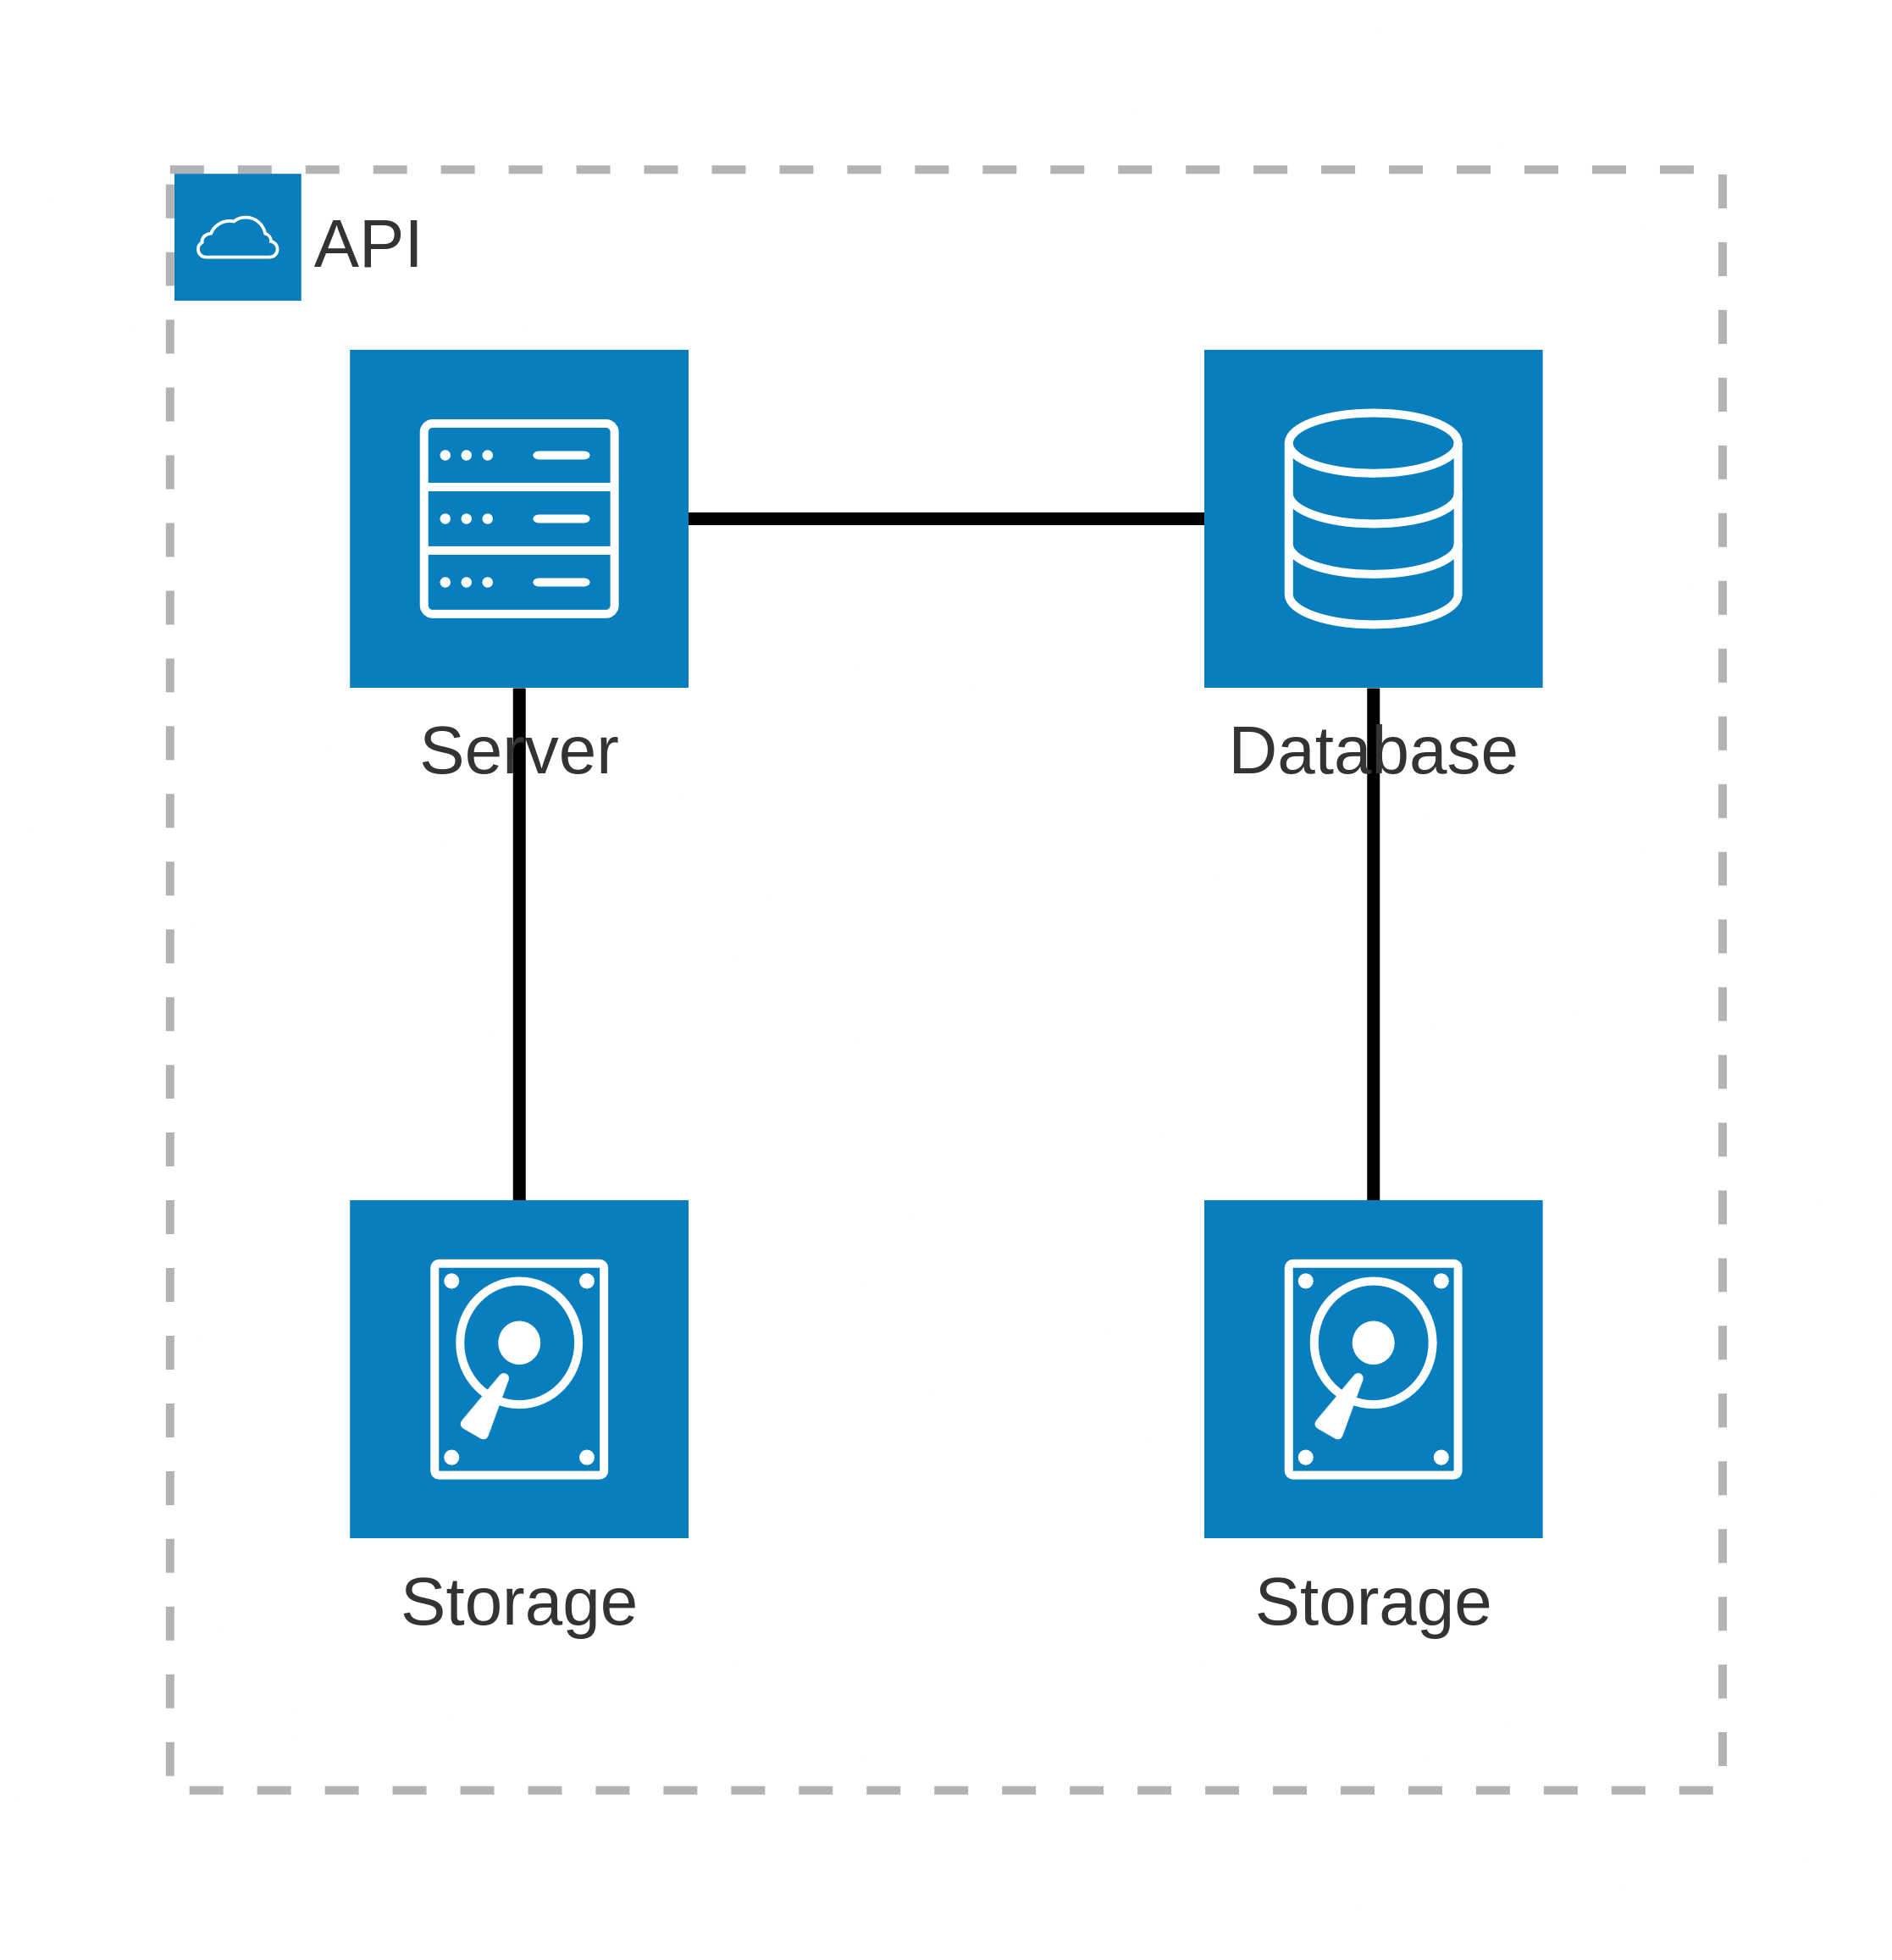
\includegraphics[width=0.5\textwidth]{../graphics/archplan_vb_mermaid.png}
  \caption[Voorbeeld architectuurplan in afbeeldingsformaat (\emph{MermaidJS})]{Afbeeldingsformaat voor een voorbeeld van een architectuurplan, uitgedrukt in \emph{MermaidJS} \autocite{Mermaid2026}.}
\end{figure}

\section{\emph{Infrastructure-as-Code}}%

\emph{Infrastructure-as-Code} (afgekort \emph{IaC}) is een praktijk binnen DevOps waarbij de nodes (fysiek of virtueel) binnen een IT-infrastructuur gedefinieerd en beheerd worden via machine-leesbare configuratiebestanden in plaats van via handmatige configuratie of grafische beheerconsoles \autocite{Rahman2019}.

Deze definities worden doorgaans onder versiebeheer geplaatst, waardoor men infrastructuurwijzigingen kan testen, herzien en eventueel terugdraaien zoals bij traditionele softwarecode.

De belangrijkste voordelen van \emph{IaC} zijn reproduceerbaarheid (omgevingen kunnen opnieuw identiek worden uitgerold), consistentie (vermindering van menselijke fouten en configuratiedrift), en een hogere snelheid van oplevering doordat de provisioning sterk geautomatiseerd wordt \autocite{Artac2017}.

\emph{IaC} staat echter niet in voor het configureren van nodes, dat is de taak van ``\emph{configuration management}''-tools zoals \emph{Ansible}, \emph{Puppet} en \emph{Chef}.

\textcite{Baer2025} onderscheidt grofweg twee benaderingen tot deze praktijk: een imperatieve stijl, waarin stap-voor-stap wordt beschreven welke acties er moeten worden uitgevoerd, en een declaratieve stijl, waarin enkel de gewenste eindsituatie van de infrastructuur wordt beschreven.
Moderne \emph{IaC}-tools zoals \emph{Terraform}, \emph{OpenTofu} en \emph{Vagrant} volgen hoofdzakelijk een declaratief model.

\subsection{\emph{Terraform}}%

\emph{Terraform} is een open-source ``\emph{Infrastructure-as-Code}'' tool van \emph{HashiCorp}, ontworpen om infrastructuur geautomatiseerd te provisioneren en te beheren over (meerdere) cloud- en on-premises platformen.
In plaats van infrastructuur handmatig aan te maken in een webconsole, definieert men de gewenste toestand in configuratiebestanden, waarna \emph{Terraform} aan de hand van verscheidene \emph{API}'s voor de betrokken platformen de nodige resources aanmaakt, wijzigt of verwijdert. \autocite{HashiCorp2024}

De configuraties worden geschreven in \emph{HashiCorp} Configuration Language (\emph{HCL}) (met ``\texttt{.tf}'' als bestandsextensie), een menselijk leesbare, declaratieve taal waarin men verschillende zaken kan definiëren zoals resources (zoals al dan niet virtuele nodes, maar ook bijvoorbeeld netwerken of \emph{DNS}-records), data sources (om externe data aan te reiken) en modules (sets van configuratiebestanden). \autocite{HashiCorp2025}

\emph{Terraform} ondersteunt honderden providers; dit varieert van providers ontwikkeld door officiële partners (zoals IBM en \emph{Ansible}) tot providers van third-party bedrijven (zoals \emph{Amazon AWS}, \emph{Microsoft Azure}, \emph{Google Cloud}, \ldots), wat het bijzonder flexibel maakt voor multi-cloud- en hybride omgevingen. \autocite{HashiCorp2025a}

Het volgende codefragment licht de structuur van \emph{HCL} toe via een eenvoudige topologie voor een \emph{AWS}-gebaseerde omgeving.

\begin{codeblock}
  \begin{minted}{terraform}
terraform {
  required_providers {
    aws = {
      source  = "hashicorp/aws"
      version = "~> 1.0.4"
    }
  }
}

variable "aws_region" {}

variable "base_cidr_block" {
  description = "A /16 CIDR range definition, such as 10.1.0.0/16, that the VPC will use"
  default = "10.1.0.0/16"
}
variable "availability_zones" {
  description = "A list of availability zones in which to create subnets"
  type = list(string)
}
provider "aws" {
  region = var.aws_region
}
resource "aws_vpc" "main" {
  # Referencing the base_cidr_block variable allows the network address
  # to be changed without modifying the configuration.
  cidr_block = var.base_cidr_block
}
resource "aws_subnet" "az" {
  # Create one subnet for each given availability zone.
  count = length(var.availability_zones)

  # For each subnet, use one of the specified availability zones.
  availability_zone = var.availability_zones[count.index]

  # By referencing the aws_vpc.main object, Terraform knows that the subnet
  # must be created only after the VPC is created.
  vpc_id = aws_vpc.main.id

  # Built-in functions and operators can be used for simple transformations of
  # values, such as computing a subnet address. Here we create a /20 prefix for
  # each subnet, using consecutive addresses for each availability zone,
  # such as 10.1.16.0/20 .
  cidr_block = cidrsubnet(aws_vpc.main.cidr_block, 4, count.index + 1 )
}
\end{minted}
  \caption[Voorbeeld \emph{Terraform}-configuratie]{Voorbeeld van een eenvoudige \emph{Terraform}-configuratie \autocite{HashiCorp2025}.}
  \label{code:terraform_vb}
\end{codeblock}

\subsection{\emph{OpenTofu}}%

\emph{OpenTofu} is een relatief recente speler, ontstaan als een community-gedreven fork van \emph{Terraform} in 2023. De drijfveer achter deze fork is de keuze van \emph{HashiCorp} om een licentiewijziging naar het \emph{Business Source License} (afgekort \emph{BSL}) voor \emph{Terraform} door te voeren. Dit bracht het bestuur in gevaar voor de bestaande community, die op lange termijn eerder leveranciersonafhankelijk willen blijven. \autocite{Gaddam2023}

Het project heeft als doel een volledig vrije, open-governance variant van de \emph{Terraform}-tooling te bieden, met langdurige compatibiliteit en transparante besluitvorming in de open-source gemeenschap.

Op technisch vlak positioneert \emph{OpenTofu} zich als een drop-in replacement voor \emph{Terraform 1.6.x} (en voorafgaande versies); bestaande configuraties in \emph{HCL} en de bekende \emph{CLI}-commando's blijven bruikbaar, zodat organisaties en projecten relatief eenvoudig kunnen migreren zonder hun codebase volledig te moeten herschrijven.
De tool ondersteunt dus dezelfde concepten (providers, resources, modules en state-bestanden) en streeft naar \emph{backwards compatibility}, terwijl op termijn nieuwe functionaliteit kan worden geïntroduceerd die niet noodzakelijk in \emph{Terraform} beschikbaar is. \autocite{OpenTofu2026}

\subsection{\emph{Vagrant}}%

\emph{Vagrant} is een tool van \emph{HashiCorp} voor het bouwen en beheren van (lokale) virtuele omgevingen via een tekstueel configuratiebestand (``\texttt{Vagrantfile}'').
Het doel van \emph{Vagrant} is om reproduceerbare ontwikkel- en testomgevingen te creëren die met één commando kunnen opgestart, geprovisioneerd en opnieuw vernietigd worden. \autocite{HashiCorp2026}

In de ``\texttt{Vagrantfile}'' specificeert men voor elke virtuele machine, onder andere, de base box (of het gastbesturingssysteem zoals \emph{AlmaLinux}, Alpine Linux, Ubuntu), het aantal \emph{CPU} cores, hoeveelheid werkgeheugen, welke netwerkconfiguratie van toepassing is, en welke provisioning-stappen moeten worden uitgevoerd.
Standaard ondersteunt \emph{Vagrant} providers zoals \emph{VirtualBox}, \emph{Hyper-V} en \emph{Docker}, maar via plugins kunnen ook andere platformen worden aangestuurd, waaronder \emph{VMware} of publieke cloudproviders. \autocite{HashiCorp2026a}

Voor provisioning kan \emph{Vagrant} gebruik maken van verschillende methodes zoals \emph{Bash}-scripts maar ook ``\emph{configuration management}''-tools (\emph{Ansible}/\emph{Chef}/\emph{Puppet}).
Dit maakt het mogelijk om via het ``\texttt{vagrant up}''-commando zowel de virtuele infrastructuur (via \emph{Vagrant}) als de configuratie van het gastbesturingssysteem (bijvoorbeeld via \emph{Ansible}-\emph{playbooks}) te automatiseren. \autocite{HashiCorp2026a}

Binnen de opleiding \emph{Toegepaste Informatica} wordt \emph{Vagrant} ingezet om snel identieke virtuele omgevingen uit te rollen waarin \emph{Ansible} de verdere configuratie en deployment van software verzorgt.

Het volgende codefragment licht een mogelijke, eenvoudige ``\texttt{Vagrantfile}'' toe.

\begin{codeblock}
  \begin{minted}{ruby}
Vagrant.configure("2") do |config|
  config.vm.box = "hashicorp-education/ubuntu-24-04"
  config.vm.box_version = "0.1.0"
  # Install Docker and dependencies
  config.vm.provision "shell", name: "install-dependencies", path: "install-dependencies.sh"
  # Start Terramino (can be rerun with vagrant provision --provision-with start-terramino)
  config.vm.provision "shell", name: "start-terramino", inline: <<-SHELL
    cd /home/vagrant/terramino-go
    docker compose up -d
  SHELL
  # Restart Terramino (can be rerun with vagrant provision --provision-with restart-terramino)
  # For quick changes that doesn't require rebuilding (e.g. frontend changes)
  config.vm.provision "shell", name: "restart-terramino", run: "never", inline: <<-SHELL
    docker compose restart
  SHELL
  # Reload Terramino (can be rerun with vagrant provision --provision-with reload-terramino)
  # For changes that require rebuilding (e.g. backend changes)
  config.vm.provision "shell", name: "reload-terramino", run: "never", inline: <<-SHELL
    /usr/local/bin/reload-terramino
  SHELL
end
\end{minted}
  \caption[Voorbeeld ``\texttt{Vagrantfile}'']{Voorbeeld van een eenvoudige ``\texttt{Vagrantfile}'' \autocite{HashiCorp2024a}.}
  \label{code:vagrantfile_vb}
\end{codeblock}

\section{\emph{Configuration management}}%

\emph{Configuration management} is het principe om een (grote) set van manuele, repetitieve configuratietaken (installeren van \emph{packages}, beheren van \emph{firewalls}, instellen van de default gateways en \emph{DNS}-servers, \ldots) automatisch te laten uitvoeren op servers. In het beste geval verloopt dit proces op een idempotente manier; op basis van dezelfde stappen wordt hetzelfde resultaat opgeleverd zonder afwijkingen, en vertoont het proces dus consistent gedrag. Deze manier van werken, analoog met het principe van \emph{Infrastructure-as-Code}, schaalt beter voor omgevingen met honderden of duizenden nodes, aangezien het aanzienlijk minder tijdrovend en vatbaar voor menselijke fouten is. \autocite{Likitha2022}

Als \emph{Infrastructure-as-Code} een omgeving automatisch opzet, staat \emph{configuration management} met andere woorden in voor het configuratie-aspect.

\emph{Ansible}, \emph{Puppet} en \emph{Chef} zijn drie open-source tools die in de praktijk het meest gebruikt worden om \emph{configuration management} toe te passen \autocite{Masek2018}.

\subsection{\emph{Ansible}}%

\emph{Ansible} is een open-source ``\emph{configuration management}''-tool die werkt zonder permanente \emph{agents} op de doelhosts: standaard maakt het verbinding via \emph{SSH} om taken uit te voeren.
Beheerders beschrijven de gewenste configuratie in menselijk leesbare YAML-bestanden, zogenaamde \emph{playbooks}, die bestaan uit taken (\emph{tasks}) en herbruikbare rollen (\emph{roles}). \autocite{Ansible2025}

Taken maken gebruik van (ingebouwde) modules om verscheidene systeem-gerelateerde objecten te beheren, zoals \emph{packages}, \emph{services}, gebruikers, bestanden en \emph{firewall}-regels.
Hier is de kracht van \emph{Ansible} dat men deze taken op declaratieve wijze kan schrijven in plaats van imperatief; men beschrijft \emph{wat} het eindresultaat moet zijn, niet \emph{hoe} men daar moet geraken. \emph{Ansible} biedt hier dus ook de mogelijkheid om \emph{playbooks} zo idempotent mogelijk te schrijven; bij herhaalde uitvoeringen krijgt men steeds hetzelfde, verwachte eindresultaat. \autocite{Stoeckl2025}

Dankzij een \emph{inventory}-bestand kunnen de taken van een \emph{playbook} identiek uitgevoerd worden op groepen van meerdere hosts, wat \emph{Ansible} geschikt maakt voor het configureren van tientallen of honderden servers in één keer. \autocite{Ansible2025}

Onderstaand voorbeeld toont een beknopte \emph{Ansible}-\emph{playbook} die twee taken uitvoert: de webserver en databankserver updaten op alle hosts in de overeenkomende groepen (``\texttt{webservers}'' en ``\texttt{databases}'').

\begin{codeblock}
  \begin{minted}{yaml}
---
- name: Update web servers
  hosts: webservers
  remote_user: root

  tasks:
  - name: Ensure apache is at the latest version
    ansible.builtin.yum:
      name: httpd
      state: latest

  - name: Write the apache config file
    ansible.builtin.template:
      src: /srv/httpd.j2
      dest: /etc/httpd.conf

- name: Update db servers
  hosts: databases
  remote_user: root

  tasks:
  - name: Ensure postgresql is at the latest version
    ansible.builtin.yum:
      name: postgresql
      state: latest

  - name: Ensure that postgresql is started
    ansible.builtin.service:
      name: postgresql
      state: started
\end{minted}
  \caption[Voorbeeld \emph{Ansible}-\emph{playbook}]{Voorbeeld van een eenvoudige \emph{Ansible}-\emph{playbook} \autocite{Ansible2025a}.}
  \label{code:ansible_playbook_vb}
\end{codeblock}

Deze \emph{playbook} kan herhaaldelijk uitgevoerd worden en telkens hetzelfde resultaat opleveren, wat het potentieel van \emph{Ansible} qua idempotentie (zeker voor de ingebouwde modules) illustreert.

\subsection{\emph{Puppet}}%

\emph{Puppet} is een ``\emph{configuration management}''- tool die gebruikmaakt van een declaratieve domeinspecifieke taal (gebaseerd op \emph{Ruby}) om de gewenste toestand van systemen te beschrijven.
Beheerders definiëren resources (zoals \emph{packages}, files en \emph{services}) in \emph{manifests}; \emph{Puppet} vergelijkt vervolgens de actuele toestand van een host met deze gewenste toestand en brengt enkel de noodzakelijke wijzigingen aan. \autocite{Perforce2026a}

Typisch wordt \emph{Puppet} ingezet in een ``\emph{server-agent}''-architectuur: een centrale \emph{Puppet}-server compileert de \emph{manifests} tot een \emph{catalog} en deelt deze catalog uit aan \emph{Puppet}-\emph{\emph{agent}s} op de beheerde hosts.
De \emph{agent} past de catalog toe, corrigeert eventuele configuratiedrift en rapporteert zijn status terug aan de server, waardoor beheerders op grote schaal configuraties kunnen afdwingen en monitoren. \autocite{Perforce2026b}

Het volgende \emph{manifest} toont vereenvoudigd aan hoe een server geconfigureerd kan worden met \emph{Puppet}:

\begin{codeblock}
  \begin{minted}{ruby}
file { 'ntp.conf':
  path    => '/etc/ntp.conf',
  ensure  => file,
  content => template('ntp/ntp.conf'),
  owner   => 'root',
  mode    => '0644',
}

package { 'ntp':
  ensure => installed,
  before => File['ntp.conf'],
}

service { 'ntpd':
  ensure    => running,
  subscribe => File['ntp.conf'],
}
\end{minted}
  \caption[Eenvoudig \emph{Puppet}-\emph{manifest} voor een webserver]{\autocite{Perforce2026}}
  \label{code:puppetvb}
\end{codeblock}

Wanneer de \emph{agent} dit \emph{manifest} meerdere keren toepast, zal \emph{Puppet} enkel wijzigingen maken als de werkelijke toestand (bijvoorbeeld ontbrekende bestanden of een gestopte \emph{service}) afwijkt van de beschreven gewenste toestand.

\subsection{\emph{Chef}}%

\emph{Chef} is een ``\emph{configuration management}''-tool en automatiseringsplatform dat \emph{Infrastructuur-as-Code} benadert via \emph{Ruby}-gebaseerde code.
Configuratie wordt georganiseerd in \emph{cookbooks}, die één of meerdere \emph{recipes} bevatten; een \emph{recipe} beschrijft met behulp van resources (zoals ``\texttt{package}'', ``\texttt{file}'' en ``\texttt{service}'') de gewenste toestand van een node.  \autocite{ProgressSoftware2026}

In een typische opstelling communiceren \emph{Chef}-clients op de beheerde nodes met een centrale \emph{Chef}-server, die \emph{cookbooks}, policies en \emph{run lists} beheert.
Tijdens een \emph{run} vraagt de client zijn \emph{run list} op, convergeert het systeem naar de in de \emph{recipes} gedefinieerde toestand en rapporteert het resultaat terug, wat een idempotente, herhaalbare configuratieworkflow oplevert. \autocite{ProgressSoftware2026a}

Onderstaande vereenvoudigde \emph{recipe} installeert een \emph{Apache} webserver, kiest op willekeurige basis \emph{PHP} of \emph{Perl} als scriptingtaal, en installeert deze vervolgens.

\begin{codeblock}
  \begin{minted}{ruby}
package 'httpd' do
  action :install
end

ruby_block 'randomly_choose_language' do
  block do
    if Random.rand > 0.5
      node.run_state['scripting_language'] = 'php'
    else
      node.run_state['scripting_language'] = 'perl'
    end
  end
end

package 'scripting_language' do
  package_name lazy { node.run_state['scripting_language'] }
  action :install
end
\end{minted}
  \caption[Eenvoudige \emph{Chef}-\emph{recipe} voor een webserver]{\autocite{ProgressSoftware2025}}
  \label{code:chefvb}
\end{codeblock}

Bij elke \emph{Chef}-\emph{run} wordt deze \emph{recipe} opnieuw geëvalueerd; als ``\texttt{httpd}'' al geïnstalleerd is en de client overeenkomt met de gewenste toestand, zullen er geen wijzigingen meer worden doorgevoerd, in lijn met het idempotente karakter van \emph{configuration management}. Als bij de volgende \emph{run} een andere scriptingtaal wordt gekozen, dan zullen de wijzigingen op basis daarvan uitgevoerd worden (de deinstallatie van de oude scriptingtaal, gevolgd door installatie van de nieuwe scriptingtaal).

\section{De opleiding Toegepaste Informatica (\emph{HOGENT})}%
\label{sec:opleiding}

\emph{Toegepaste Informatica} is een professionele bacheloropleiding van drie jaar aan \emph{HOGENT}, aangeboden door het \emph{Departement IT \& Digitale Innovatie} \autocite{HOGENT2024}. In het derde jaar kiezen studenten een keuzeprofiel dat aansluit bij hun interesse; voor studenten met een interesse in serverinfrastructuur, netwerken en automatisering is dat het keuzeprofiel ``\emph{IT infrastructure engineer}''.

De volgende subsecties beschrijven achtereenvolgend het relevante keuzeprofiel (``\emph{IT infrastructure engineer}''), drie \emph{OLODs} (opleidingsonderdelen) die er binnen vallen en centraal staan in deze bachelorproef, de \emph{Ansible}-rollen en de \emph{Ansible Skeleton} van Bert Van Vreckem, en tot slot een algemeen overzicht van de voornaamste tools die binnen de \emph{OLODs} in dit keuzeprofiel worden ingezet.

\subsection{``IT infrastructure engineer'' (Keuzeprofiel)}%
\label{subsec:keuzeprofiel}

Binnen dit keuzeprofiel zijn er drie \emph{OLODs} die relevant zijn voor deze bachelorproef, omdat ze elk op hun manier het ontwerpen en/of implementeren van virtuele serverinfrastructuren centraal stellen:

\begin{itemize}
  \item ``\emph{Cybersecurity Advanced}'' \autocite{HOGENT2025}
  \item ``\emph{Infrastructure Automation}'' \autocite{HOGENT2025a}
  \item ``\emph{DevOps Project: Operations}'' \autocite{HOGENT2025b}
\end{itemize}

De twee eerstgenoemde \emph{OLODs} stellen hierbij een initiële labo-omgeving beschikbaar via de \emph{GitHub}-organisatie \emph{HoGentTIN} \autocite{HoGentTIN2025,HoGentTIN2025a}. In elk van deze \emph{OLODs} wordt een basisinfrastructuur aangeboden waarop studenten verder kunnen bouwen; hoe deze infrastructuur opgezet, geconfigureerd en gedocumenteerd wordt, is telkens een kerndoelstelling van het \emph{OLOD}.

\subsection{``\emph{Cybersecurity Advanced}'' (\emph{OLOD})}%
\label{subsec:cybersec_adv}

Het \emph{OLOD} ``\emph{Cybersecurity Advanced}'' introduceert het concept van ``\emph{blue-teaming}'' -- het verdedigen van een netwerk tegen aanvallen -- aan de hand van een reeks virtuele labo's die individueel worden uitgevoerd \autocite{HOGENT2025}. De labo's draaien telkens rond een basisomgeving met meerdere virtuele machines die elk een specifieke rol opnemen (\emph{DNS}-server, webserver, databankserver, \ldots).

Het gebruik van \emph{configuration management} of \emph{UML}-diagrammen is hierbij niet strikt noodzakelijk, maar het geeft de student een aanzienlijk voordeel: de labo-omgeving is zo overzichtelijker en kan (na het manueel uitvoeren van elk labo) snel opnieuw opgezet worden met de relevante aanpassingen. De initiële labo-omgeving wordt alvast voorgesteld met een netwerkdiagram ontworpen via \emph{PlantUML} \autocite{HoGentTIN2025}, wat studenten een rechtstreekse link biedt tussen het diagram en de effectieve omgeving.

\subsection{``\emph{Infrastructure Automation}'' (\emph{OLOD})}%
\label{subsec:infra_auto}

``\emph{Infrastructure Automation}'' is een \emph{OLOD} dat een reeks labo's bevat die verschillende tools introduceren voor het automatisch opzetten, configureren en monitoren van serveromgevingen, waaronder \emph{Ansible}, \emph{Jenkins}\footnote{\url{https://www.jenkins.io/}}, \emph{Prometheus}\footnote{\url{https://prometheus.io/}} en \emph{Kubernetes}\footnote{\url{https://kubernetes.io/}} \autocite{HOGENT2025a}. In tegenstelling tot ``\emph{Cybersecurity Advanced}'' is het gebruik van \emph{configuration management} hier een centrale leerdoelstelling: de labo's vereisen dat studenten \emph{Ansible} inzetten om de virtuele machines te configureren.

De labo-omgeving voor dit \emph{OLOD} is gebaseerd op de ``\emph{Ansible Skeleton}'' van \textcite{Vreckem2025}: een sjabloon voor \emph{Ansible}-projecten met een geïntegreerde \emph{Vagrant}-omgeving (zie \autoref{subsec:bertvv}). Deze structuur -- met mappen zoals ``\texttt{ansible/}'', ``\texttt{ansible/host\_vars/}'', ``\texttt{ansible/group\_vars/}'' en een centrale ``\texttt{site.yml}''-\emph{playbook} -- vormt ook de uitvoerstructuur van de \emph{converter} die in deze bachelorproef wordt ontwikkeld \autocite{HoGentTIN2025a}.

\subsection{``\emph{DevOps Project: Operations}'' (\emph{OLOD})}%
\label{subsec:devops_ops}

``\emph{DevOps Project: Operations}'' is een \emph{OLOD} dat het tweede luik vormt van een tweeledig groepsproject \autocite{HOGENT2025b}, het eerste luik zijnde ``\emph{Real-life Integrated Software Engineering}'' (\emph{RISE}) voor de studenten binnen het keuzetraject ``\emph{full stack developer}''.
Het doel van het ``\emph{operations}-team'' is om de backend van een webapplicatie (bijvoorbeeld een \emph{.NET}- of \emph{Android}-\emph{package}) -- ontwikkeld door een parallel ``\emph{development}-team'' -- te ondersteunen met een productie-waardige serverinfrastructuur. Deze omgeving moet volledig geautomatiseerd kunnen opgezet worden via \emph{Infrastructure-as-Code}- en \emph{configuration management}-tools.

In tegenstelling tot de twee vorige \emph{OLODs} is het gebruik van een netwerkdiagram hier verplicht: de onderliggende architectuur moet gevisualiseerd worden voor zowel technische als niet-technische stakeholders via \emph{UML}-modelleringssoftware. Dit \emph{OLOD} combineert daarmee twee aspecten die centraal staan in deze bachelorproef: het ontwerpen van een infrastructuur via (\emph{UML}-)diagrammen, en het automatisch uitrollen ervan via \emph{IaC} en \emph{configuration management}.

\subsection{\emph{Ansible}-rollen en \emph{Ansible Skeleton} van Bert Van Vreckem}%
\label{subsec:bertvv}

Een aantal centrale bouwstenen binnen de bovenstaande \emph{OLODs} -- en bij uitbreiding binnen de \emph{converter} ontwikkeld in deze bachelorproef -- zijn de \emph{Ansible}-rollen en \emph{Ansible Skeleton} van \textcite{Vreckem2025}.
De \emph{Ansible Skeleton} is een sjabloon voor \emph{Vagrant}- en \emph{Ansible}-projecten dat een vaste mappenstructuur, een vooraf geconfigureerde ``\texttt{Vagrantfile}'' en hulpscripts omvat. Deze ``\texttt{Vagrantfile}'' is zo ontworpen zodat men enkel in een apart ``\texttt{vagrant-hosts.yml}''-bestand hosts moet definiëren om deze vervolgens eenvoudig op te starten met het ``\texttt{vagrant up}''-commando.

Naast de \emph{Ansible Skeleton} heeft \textcite{Vreckem2016} ook een reeks \emph{Ansible}-rollen ontwikkeld die specifiek gericht zijn op \emph{RedHat}-gebaseerde distributies en die binnen de opleiding standaard worden ingezet, waarvan hier enkele voorbeelden:

\begin{description}
  \item[``\texttt{bertvv.rh-base}''] Basisinstallatie en -configuratie van een \emph{RedHat}-gebaseerde server: \emph{firewall}, \emph{SELinux}, gebruikersbeheer en algemene systeeminstellingen \autocite{Vreckem2016}.
  \item[``\texttt{bertvv.bind}''] Installatie en configuratie van \emph{BIND9} als autoritatieve \emph{DNS}-server \autocite{Vreckem2015}.
  \item[``\texttt{bertvv.dhcp}''] Installatie en configuratie van \emph{ISC DHCP} als \emph{DHCP}-server \autocite{Vreckem2015a}.
  \item[``\texttt{bertvv.httpd}''] Installatie en configuratie van een \emph{Apache}-webserver \autocite{Vreckem2015b}.
\end{description}

\subsection{Overzicht voornaamste tools}%
\label{subsec:overzicht_tools}

De volgende tabel geeft een algemeen overzicht van de voornaamste tools die voor de bovenstaande \emph{OLODs} (binnen het keuzeprofiel ``\emph{IT infrastructure engineer}'') worden ingezet, alsook de context waarin ze worden gebruikt:

\begin{table}[H]
  \centering
  \begin{tabularx}{\textwidth}{l X}
    \toprule
    \textbf{Tool}                           & \textbf{Context}                                                       \\
    \midrule
    \emph{Visual Paradigm} / \emph{draw.io} & Ontwerp van netwerk- en \emph{UML}-diagrammen (\emph{GUI}-gebaseerd)   \\
    \emph{PlantUML}                         & Tekstueel diagramformaat (aangeraden in \emph{Cybersecurity Advanced}) \\
    \emph{Vagrant}                          & \emph{IaC} voor lokale VM-omgevingen (via \emph{Ansible Skeleton})     \\
    \emph{Ansible}                          & ``\emph{Configuration management}''-tool van virtuele machines         \\
    \emph{Git} / \emph{GitHub}              & Versiebeheer van code en documentatie voor projecten en labo's         \\
    \bottomrule
  \end{tabularx}
  \caption[Overzicht van voornaamste tools binnen keuzeprofiel ``\emph{IT infrastructure engineer}'']{Overzicht van de voornaamste tools die worden ingezet binnen de \emph{OLODs} uit het keuzeprofiel ``\emph{IT infrastructure engineer}''.}
  \label{tab:overzicht_tools}
\end{table}

\section{\emph{Compilers}}%
\label{sec:compilers}

\emph{Compilers} vertalen de broncode van een \emph{high-level}, menselijk leesbare taal (zoals \emph{Java}\footnote{\url{https://www.java.com/}} of \emph{C\#}\footnote{\url{https://dotnet.microsoft.com/en-us/languages/csharp}}) tot equivalente instructies in een andere, vaak \emph{low-level} taal of machinecode \autocite{Seidl2012}. Dit proces verloopt in meerdere opeenvolgende fases, waarbij elke fase de uitvoer van de vorige als invoer neemt.

\subsection{Fases}%
\label{subsec:compilerfases}

\subsubsection{Lexicale analyse}%

De eerste fase, de \emph{lexicale analyse} (ook wel ``\emph{scanning}'' of ``\emph{tokenisatie}'' genoemd), leest de broncode karakter per karakter en groepeert deze in betekenisvolle eenheden of ``\emph{tokens}'' \autocite{Seidl2012}. Voorbeelden van \emph{tokens} zijn sleutelwoorden (``\texttt{if}'', ``\texttt{while}''), identifiers, operatoren en literals. Witruimte en commentaar wordt hier doorgaans geen rekening mee gehouden, tenzij de brontaal in kwestie bijvoorbeeld wel witruimte-gevoelig is (zoals bij \emph{Python}).

\subsubsection{\emph{Parsen}/ontleden}%

De \emph{parser} neemt de \emph{tokens} van de vorige fase als invoer en controleert of deze voldoen aan de grammaticale regels van de brontaal \autocite{Seidl2012}. Het resultaat is een \emph{parse tree}, die de hiërarchische structuur van de broncode weergeeft (zie \autoref{subsec:parsetree}). Als de \emph{tokens} niet grammaticaal correct zijn, ontstaat er in de \emph{parser} een syntaxfout.

\subsubsection{Semantische analyse}%

Waar de \emph{parser} enkel de syntactische correctheid controleert, gaat de \emph{semantische analyse} na of de code ook effectief betekenisvol is \autocite{Seidl2012}. Typische controles zijn typeverificatie, scopecontrole en het oplossen van namen. Het resultaat is doorgaans een verrijkte \emph{abstracte syntaxboom} (of \emph{AST}, zie \autoref{subsec:ast}).

\subsubsection{Optimalisatie}%

De optionele \emph{optimalisatiefase} transformeert de tussentijdse representatie om de efficiëntie van de gegenereerde code te verbeteren, zonder de semantiek te wijzigen \autocite{Seidl2012}. Voorbeelden zijn \emph{constant folding}, het elimineren van dode code en het \emph{inlinen} van kleine functies.

\subsubsection{Codegeneratie}%

De laatste fase zet de (al dan niet geoptimaliseerde) tussentijdse representatie om naar de doeltaal \autocite{Seidl2012}. Voor traditionele \emph{compilers} is dit machinecode of \emph{Assembly}; voor andere \emph{compilers} kan dit ook een andere \emph{high-level} taal zijn. In dat laatste geval spreekt men van een \emph{transpiler}, wat in \autoref{sec:transpilers} verder wordt toegelicht.

\subsection{Abstract Syntax Tree (\emph{AST})}%
\label{subsec:ast}

Een \emph{Abstract Syntax Tree} (afgekort \emph{AST}) is een boomstructuur die de logische, abstracte structuur van de broncode weergeeft, zonder overbodige grammaticale details zoals haakjes of scheidingstekens \autocite{Freitas2025}. Elke knoop in de boom stelt een constructie uit de broncode voor (zoals een expressie of declaratie), terwijl de bladeren de concrete waarden bevatten. \emph{Compilers} gebruiken de \emph{AST} als centrale tussentijdse representatie: de invoertaal wordt geparsed naar een \emph{AST}, getransformeerd, en vervolgens gegenereerd naar de doeltaal.

\subsection{\emph{Parse Tree}}%
\label{subsec:parsetree}

Een \emph{parse tree} (ook wel \emph{concrete syntaxboom}) is het directe resultaat van het \emph{parsen} van broncode en bevat \emph{alle} grammaticale informatie, inclusief interpunctie en andere syntactische details die voor de betekenis niet relevant zijn \autocite{Freitas2025}. Een \emph{AST} is in de praktijk een vereenvoudigde versie van de \emph{parse tree} waarbij de overbodige knopen zijn weggelaten. De \emph{AST} is voor \emph{transpilers} de voorkeur, omdat transformaties erop eenvoudiger en minder foutgevoelig zijn.

\section{\emph{Transpilers}}%
\label{sec:transpilers}
``\emph{Source-to-source compilers}'', algemeen gekend als ``\emph{transpilers}'', zijn \emph{compilers} die broncode geschreven in één \emph{high-level} taal omzetten naar code in een andere \emph{high-level} taal \autocite{Freitas2025}. Bekende toepassingen zijn de omzetting van moderne \emph{JavaScript} (ES2022+) naar oudere versies voor browsercompatibiliteit (via tools zoals \emph{Babel}\footnote{\url{https://babeljs.io/}}) \autocite{Nicolini2024}, de compilatie van \emph{TypeScript} naar \emph{JavaScript}, en de omzetting van \emph{C}/\emph{C++} naar \emph{WebAssembly} (via \emph{Emscripten}\footnote{\url{https://emscripten.org/}}). Voor het automatisch genereren van lexers en parsers bestaan er gespecialiseerde tools zoals \emph{ANTLR}\footnote{\url{https://www.antlr.org/}} of ingebouwde \emph{Unix}-tools zoals \emph{Lex} en \emph{Yacc}.

\section{\emph{Converters}}%
\label{sec:converters}

Waar een \emph{transpiler} een formele pipeline doorloopt (lexicale analyse, parsing, \emph{AST}-opbouw en codegeneratie), volstaat een \emph{converter} met een patroongebaseerde transformatie van het ene bestandsformaat naar het andere, zonder een volledige semantische analyse van de invoer \autocite{Plaisted2013}. Het doel is functionele equivalentie: de uitvoer moet de informatie uit de invoer correct weergeven in het doelformaat, maar het pad ernaartoe hoeft niet via een formele grammatica te lopen.

Een \emph{converter} kan bijvoorbeeld op basis van reguliere expressies of patroonherkenning relevante elementen uit een tekstbestand extraheren en deze omzetten naar een andere structuur. Dit is een pragmatische aanpak die goed werkt wanneer de invoertaal een beperkte, voorspelbare syntax heeft en er geen volledige semantische analyse vereist is.

%%=============================================================================
%% Methodologie
%%=============================================================================

\chapter{\IfLanguageName{dutch}{Methodologie}{Methodology}}%
\label{ch:methodologie}

%% In dit hoofstuk geef je een korte toelichting over hoe je te werk bent
%% gegaan. Verdeel je onderzoek in grote fasen, en licht in elke fase toe wat
%% de doelstelling was, welke deliverables daar uit gekomen zijn, en welke
%% onderzoeksmethoden je daarbij toegepast hebt. Verantwoord waarom je
%% op deze manier te werk gegaan bent.
%% 
%% Voorbeelden van zulke fasen zijn: literatuurstudie, opstellen van een
%% requirements-analyse, opstellen long-list (bij vergelijkende studie),
%% selectie van geschikte tools (bij vergelijkende studie, "short-list"),
%% opzetten testopstelling/PoC, uitvoeren testen en verzamelen
%% van resultaten, analyse van resultaten, ...
%%
%% !!!!! LET OP !!!!!
%%
%% Het is uitdrukkelijk NIET de bedoeling dat je het grootste deel van de corpus
%% van je bachelorproef in dit hoofstuk verwerkt! Dit hoofdstuk is eerder een
%% kort overzicht van je plan van aanpak.
%%
%% Maak voor elke fase (behalve het literatuuronderzoek) een NIEUW HOOFDSTUK aan
%% en geef het een gepaste titel.

% \lipsum[21-25]

\section{Fasering van de bachelorproef}%
\label{sec:fasering_bap}

Deze bachelorproef werd uitgevoerd in de volgende fases, van 9 februari (week 1) t.e.m. 22 mei (week 15), 2026:

\begin{itemize}
  \item{\nameref{sec:fase_literatuurstudie}}
  \item{\nameref{sec:fase_evaluatie_beschikbare_tools}}
  \item{\nameref{sec:fase_ontwerp_manuele_testomgeving}}
  \item{\nameref{sec:fase_implementatie_manuele_testomgeving}}
  \item{\nameref{sec:fase_opstellen_testcases}}
  \item{\nameref{sec:fase_ontwikkeling_poc}}
  \item{\nameref{sec:fase_uitvoeren_testcases}}
\end{itemize}

Indien een fase begint met hetzelfde nummer maar eindigt met een andere letter, indiceert dit dat ze op hetzelfde moment beginnen en parallel worden uitgevoerd.

Aangezien sommige fases afhankelijk zijn van elkaar en/of korter op elkaar vallen, zullen deze voor dit document in de volgende overkoepelende hoofdstukken omvat worden:

\begin{itemize}
  \item{Hoofdstuk~\ref{ch:manuele_testomgeving}: \nameref{ch:manuele_testomgeving}}
  \item{Hoofdstuk~\ref{ch:poc}: \nameref{ch:poc}}
  \item{Hoofdstuk~\ref{ch:testcases}: \nameref{ch:testcases}}
\end{itemize}

\begin{figure}[H]
  \centering
  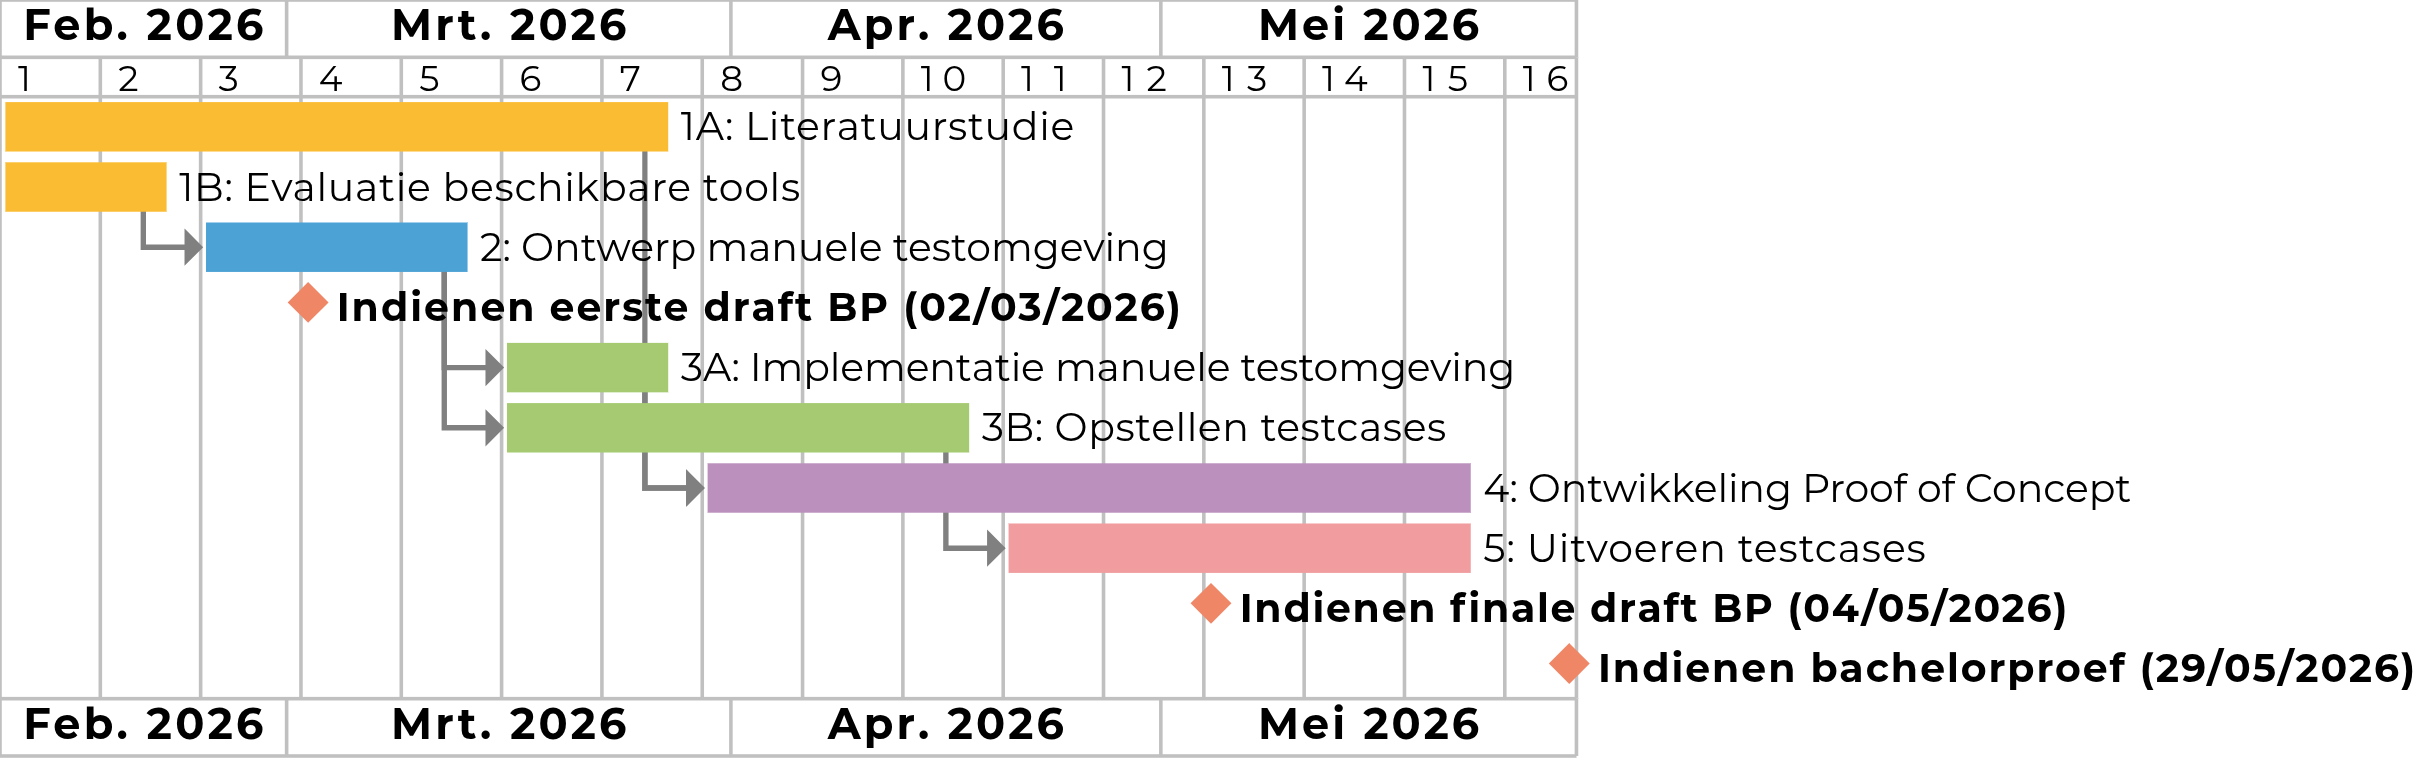
\includegraphics[width=\textwidth]{../graphics/gantt-fases.png}
  \caption[\emph{GANTT}-schema (fases van de bachelorproef)]{\label{fig:gantt-fases.png}\emph{GANTT}-schema voor de verschillende fases van de bachelorproef.}
\end{figure}

\section{Fase 1A (week 1-7): Literatuurstudie}
\label{sec:fase_literatuurstudie}

Bij het begin van het onderzoek is er parallel met de andere voorbereidende fases (1-3) een studie uitgevoerd over de stand van zaken van elk vakgebied; er werd onderzocht wat de meest courante tools zijn voor \emph{UML}-modeling, \emph{Infrastructure-as-Code} en \emph{configuration management}, alsook welke vormen de \emph{Proof of Concept} kon aannemen (zijnde als \emph{transpiler} of \emph{converter}).

\section{Fase 1B (week 1-2): Evaluatie van de beschikbare tools}%
\label{sec:fase_evaluatie_beschikbare_tools}

Hier werd er een afweging gemaakt voor de beschikbare tools  in de betrokken vakgebieden (\emph{UML}-modeling, \emph{Infrastructure-as-Code} en \emph{configuration management}) die gebruikt werden tijdens de ontwikkeling van de \emph{Proof of Concept}.
De te evalueren tools voor \emph{UML}-modeling zijn \emph{PlantUML} \& \emph{MermaidJS}, voor \emph{Infrastructure-as-Code} waren dit \emph{Terraform}, \emph{OpenTofu} \& \emph{Vagrant} en voor het ``\emph{configuration management}''-gedeelte werd er gekeken naar \emph{Ansible}, \emph{Puppet} en \emph{Chef}.

\section{Fase 2 (week 3-5): Ontwerp van de manuele testomgeving}%
\label{sec:fase_ontwerp_manuele_testomgeving}

In deze fase werd de manuele testomgeving voor de \emph{Proof of Concept} ontworpen aan de hand van netwerk- en implementatiediagrammen (ontworpen met \emph{PlantUML}/\emph{MermaidJS}). In deze diagrammen worden de hardware- (aantal \emph{CPU} cores, hoeveelheid \emph{RAM}) en softwarespecificaties (\emph{packages}, \emph{services}) van elke server beschreven, alsook hoe deze met elkaar interageren.
Deze diagrammen dienen een tweevoudig doel; ze kunnen binnen de originele context van hun taal als visuele \emph{UML}-diagrammen worden gegenereerd, en ze vormen de bron-bestanden voor de \emph{Proof of Concept}, die deze zal omzetten tot ``\emph{configuration management}''-code.

\section{Fase 3A (week 6-7): Implementatie van de manuele testomgeving}%
\label{sec:fase_implementatie_manuele_testomgeving}

Tijdens deze fase werd de infrastructuur (ontworpen in fase 2) opgezet met een \emph{Infrastructure-as-Code}-tool en geconfigureerd met een ``\emph{configuration management}''-tool (\emph{Ansible}/\emph{Puppet}/\emph{Chef}). Er werd intussen ook gedocumenteerd hoe het ``\emph{configuration management}''-gedeelte werd opgezet, want dit vormt de target output voor de \emph{Proof of Concept}.

\section{Fase 3B (week 6-10): Opstellen van de testcases}%
\label{sec:fase_opstellen_testcases}

Hier werden de testcases opgesteld waaraan de \emph{Proof of Concept} moest voldoen. Deze waren gebaseerd op bestaande omgevingen binnen de opleiding \emph{Toegepaste Informatica} en buigden zich hoofdzakelijk over de mogelijke uitvoer (de \emph{playbook}, variabelen, bestanden, \ldots) en hoe goed deze werkt tegenover de originele opstellingen.

Deze fase is in de praktijk gedeeltelijk parallel verlopen met fase 4, aangezien er tijdens het ontwikkelen van de oplossing mogelijk nieuwe testcases konden ontstaan.

\section{Fase 4 (week 8-15): Ontwikkeling van de \emph{Proof of Concept}}%
\label{sec:fase_ontwikkeling_poc}

Tijdens deze fase werd de \emph{Proof of Concept} ontwikkeld, in de vorm van een \emph{transpiler} of \emph{converter}. Deze neemt als invoer de ontworpen netwerk- en implementatiediagrammen en zet ze om tot ``\emph{Infrastructure-as-Code}''- en ``\emph{configuration management}''-code als uitvoer.

Deze fase liep tot 22 mei, 2026.

\section{Fase 5 (week 11-15): Uitvoeren van de testcases}%
\label{sec:fase_uitvoeren_testcases}

Ten slotte werden de opgestelde testen uit fase 3B uitgevoerd op de (gedeeltelijk) uitgewerkte \emph{Proof of Concept}. Op basis van de resultaten zijn er beoordelingen opgesteld die aangeeft in welke mate deze oplossing erin slaagt om een werkend eindresultaat te produceren.

Nogmaals, deze fase is parallel verlopen met fase 4.


% Voeg hier je eigen hoofdstukken toe die de ``corpus'' van je bachelorproef
% vormen. De structuur en titels hangen af van je eigen onderzoek. Je kan bv.
% elke fase in je onderzoek in een apart hoofdstuk bespreken.

%\input{...}
%\input{...}
%...

%%=============================================================================
%% Ontwerp en implementatie van de testomgeving
%%=============================================================================

\chapter{Ontwerp en implementatie van de testomgeving}%
\label{ch:testomgeving}

Alvorens de converter te ontwikkelen, werd er eerst een manuele testomgeving opgezet die als referentie dient voor de gewenste uitvoer. Dit hoofdstuk beschrijft achtereenvolgens de keuzes van elke tool die aan de basis van deze omgeving ligt, de concrete implementatie met de bijhorende Ansible- en Vagrant-configuratiebestanden, alsook hoe deze is ontworpen aan de hand van een netwerk- en implementatiediagram (in PlantUML). De converter die in het volgende hoofdstuk (\nameref{ch:poc}) wordt ontwikkeld, moet voor deze diagrammen als invoer een functioneel equivalente omgeving als uitvoer produceren.

\section{Evaluatie en toolkeuze}%
\label{sec:toolkeuze}

De keuzes voor de tools (diagramformaat, \emph{configuration management}-tool, \emph{Infrastructure-as-Code}-tool en gastbesturingssysteem) die in deze testomgeving worden ingezet, werden onder andere bepaald op basis van de aanwezigheid binnen de opleiding \emph{Toegepaste Informatica} en de praktische haalbaarheid voor de context van de converter.

\subsection{Diagramformaat (PlantUML)}%

Zoals besproken in \nameref{sec:uml}, zijn \emph{Visual Paradigm} en \emph{draw.io} de voornaamste UML-tools binnen de opleiding, maar beide zijn GUI-gebaseerd en werken met een drag-en-drop systeem \autocite{Lu2023}, wat ze ongeschikt maakt als invoerformaat voor een converter. \emph{MermaidJS} is een tekstueel alternatief dat beter kan verwerkt worden via patroonherkenning, maar heeft geen ingebouwde ondersteuning voor het toelichten van IP-adressen \autocite{Mermaid2026}. \emph{PlantUML} werd daarom gekozen als het diagramformaat voor de invoer van de converter: het maakt ook gebruik van een declaratief tekstformaat, maar het wordt ook al reeds gebruikt om de labo-omgeving van \emph{Cybersecurity Advanced} te visualiseren \autocite{HoGentTIN2025} en het leent zich goed tot versiebeheer met Git.

\subsection{Configuration Management (Ansible)}%

Zowel \emph{Puppet} als \emph{Chef} zijn volwaardige oplossingen voor het toepassen van \emph{configuration management}, maar beiden vereisen een agent die vooraf op de beheerde hosts staat \autocite{Perforce2026a,ProgressSoftware2026}. Voor de doeleinden van deze proof-of-concept werd er gekozen voor \emph{Ansible}, omwille van de agentloze werking via SSH en de beschikbaarheid van de bestaande \emph{Ansible}-rollen en ``\emph{Ansible Skeleton}'' van \textcite{Vreckem2025} die courant binnen de opleiding gebruikt worden.

\subsection{Infrastructure-as-Code (Vagrant)}%

Terraform en OpenTofu zijn krachtigere ``\emph{Infrastructure-as-Code}''-tools voor cloud- en multi-platform omgevingen, maar vallen qua functionaliteit ver buiten de scope van lokale testomgevingen die binnen de opleiding opgezet worden \autocite{HashiCorp2026}. \emph{Vagrant} werd daarom als IaC-backend ingezet, alsook omdat het naadloos integreert met de ``\emph{Ansible Skeleton}'', die hier al gebruik van maakt.

\subsection{Gastbesturingssysteem (AlmaLinux 9)}%

Als gastbesturingssysteem (voor de op te zetten VM's) werd er gekozen voor \emph{AlmaLinux 9}. De reden hierachter is eerder een compatibiliteitsprobleem: de \emph{Ansible}-rollen van \textcite{Vreckem2016} zijn ontwikkeld voor oudere versies van Ansible die op \emph{AlmaLinux 10} niet volledig worden ondersteund, waardoor de functionaliteit ervan beperkt of verhinderd wordt. Deze keuze heeft uiteraard implicaties voor de veiligheid van de omgeving op lange termijn, maar is voor de doeleinden van deze proof-of-concept een aanvaardbare afweging.

\section{Ontwerp van de testomgeving}%
\label{sec:ontwerp_testomgeving}

\subsection{Rollen}%

De testomgeving bestaat uit drie virtuele machines, elk met een specifieke rol. Deze rollen werden gekozen omdat ze samen een representatieve, maar beheerbare omgeving vormen die voldoende (aantoonbare) verbindingen bevat om de meerwaarde van een implementatiediagram te illustreren.

\begin{description}
    \item[\texttt{web}] De webserver (IP: ``\texttt{172.26.0.10}'') combineert ``\texttt{bertvv.httpd}'' met een MariaDB-databank om een simpele \emph{PHP}-pagina te hosten die met deze databank verbinding maakt. Er worden ook drie Prometheus-exporters geïnstalleerd, namelijk ``\texttt{node\_exporter}'', ``\texttt{mysqld\_exporter}'' en ``\texttt{apache\_exporter}''. Dit maakt het de meest complexe host qua geconfigureerde packages en firewallpoorten, maar met relatief weinig rechtstreekse verbindingen met andere hosts in de omgeving.
    \item[\texttt{dns}] De DNS-server (IP: ``\texttt{172.26.0.20}'') is gebaseerd op ``\texttt{bertvv.bind}'' en fungeert als autoritatieve DNS-server voor het ``\texttt{test.lan}''-domein. Elke host die gebruik maakt van deze DNS-server heeft er een ``\texttt{dns\_client}''-verbinding naar, wat resulteert in duidelijk zichtbare, betekenisvolle verbindingen in het implementatiediagram.
    \item[\texttt{monitoring}] De monitoringserver (IP: ``\texttt{172.26.0.30}'', 2 CPU, 2 GB RAM) draait Prometheus en Grafana en is de host met de meeste uitgaande verbindingen: hij haalt data op van \texttt{node\_exporter} op alle drie hosts, van ``\texttt{bind\_exporter}'' op ``\texttt{dns}'' en zowel van ``\texttt{mysqld\_exporter}'' als van ``\texttt{apache\_exporter}'' op ``\texttt{web}''. Dit web van afhankelijkheden is precies het type onderlinge relaties dat een implementatiediagram het best visualiseert en dat zonder diagram minder duidelijk zou zijn.
\end{description}

\subsection{Diagrammen}%

De omgeving wordt beschreven aan de hand van een netwerk- en implementatiediagram. Deze zijn complementair met elkaar: elk biedt een andere kijk op dezelfde omgeving, maar bevatten dus wel nog elk dezelfde hosts.

\subsubsection{Netwerkdiagram}

Het \textbf{netwerkdiagram} (``\texttt{nwdiag\_test\_env.puml}'') toont de netwerktopologie van de omgeving: de hosts met hun IP-adressen en het overkoepelende ``\texttt{test.lan}''-netwerk (``\texttt{172.26.0.0/16''}).

\begin{codeblock}
    \lstinputlisting[language=plantuml]{../plantuml/input/infra_auto_lab_2_env/nwdiag_infra_auto_lab_2_env.puml}
    \caption[Netwerkdiagram testomgeving in tekstformaat (PlantUML)]{Tekstformaat (``\texttt{nwdiag\_test\_env.puml}'') van het netwerkdiagram van de testomgeving.}
    \label{code:nwdiag_test_env.puml}
\end{codeblock}

Dit diagram kan door PlantUML gerendeerd worden tot de volgende afbeelding.

\begin{figure}[H]
  \centering
  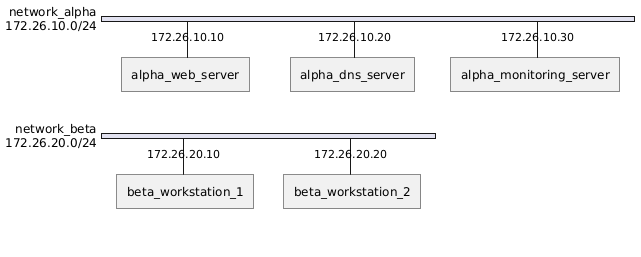
\includegraphics[width=\textwidth]{../graphics/nwdiag_test_env.png}
  \caption[Netwerkdiagram testomgeving in afbeeldingsformaat (PlantUML)]{Afbeeldingsformaat van het netwerkdiagram van de testomgeving, gegenereerd door PlantUML.}
  \label{fig:nwdiag_test_env.png}
\end{figure}

\subsubsection{Implementatiediagram}

Het \textbf{implementatiediagram} (\texttt{uml\_test\_env.puml}) toont de \emph{Ansible}-rollen die op elke host draaien en hun onderlinge verbindingen. Zo wordt in één oogopslag duidelijk welke hosts met elkaar communiceren en via welke rol. Dit diagram vormt samen met het netwerkdiagram de invoer voor de converter.

\subsection{Beperkingen}%

De volgende beperkingen gelden voor de testomgeving en bij uitbreiding voor de converter:

\begin{itemize}
\item De omgeving wordt lokaal opgezet via Vagrant en geconfigureerd via Ansible; de converter zal dus uitvoer genereren die op deze backends zijn afgestemd.
\item Enkel IPv4 wordt ondersteund bij het definiëren van netwerkadressen en host-IP's.
\item De control node (\texttt{172.26.255.253}) is aanwezig in \texttt{vagrant-hosts.yml} maar wordt niet gerepresenteerd in de netwerk- of implementatiediagrammen.
\item Routering en switching worden niet in rekening gebracht.
\end{itemize}
%%=============================================================================
%% Ontwikkeling van de Proof-of-Concept
%%=============================================================================

\chapter{Ontwikkeling van de proof-of-concept}%
\label{ch:poc}

\section{Vogelperspectief van de tool}%

<TODO>

\subsection{Ontwerpkeuzes}%

<TODO>

\subsection{Beperkingen}

<TODO>

\section{Invoer}%

<TODO>

\subsection{Formaat van het netwerkdiagram}%

<TODO>

\subsection{Formaat van het implementatiediagram}%

<TODO>

\subsection{Definitie van de (custom) rollen}

<TODO>

\section{Verwerking}%

<TODO>

\subsection{Parsering van het netwerkdiagram}%

<TODO>

\subsection{Parsering van het implementatiediagram}%

<TODO>

\section{Uitvoer}%

<TODO>

\subsection{Gekopieerde (statische) assets}%

<TODO>

\subsection{Gegenereerde (dynamische) code}%

<TODO>
%%=============================================================================
%% Opstelling en uitvoering van de testcases
%%=============================================================================

\chapter{Opstelling en uitvoering van de testcases}%
\label{ch:testcases}

Dit hoofdstuk beschrijft hoe de labo-omgevingen van de OLODs \emph{Cybersecurity Advanced} en \emph{Infrastructure Automation} zijn herontworpen als PlantUML-invoer (netwerk- en implementatiediagrammen) voor de converter. Hierna wordt dan ook telkens beschreven welke Vagrant- en Ansible-uitvoer hier telkens uit ontstaat. De selectie van hosts en rollen is gebaseerd op de originele Vagrant- en Ansible-configuraties van de betrokken labo's, maar er zullen daarin beperkingen zijn wegens de scope van de proof-of-concept.

\section{Werkwijze}%
\label{sec:werkwijze_testcases}

Voor elke testcase worden eerst de beheerde hosts uit de betrokken labo-omgevingen geïdentificeerd (op basis van de originele ``\texttt{vagrant-hosts.yml}'' en ``\texttt{inventory.yml}'') en vervolgens in het netwerkdiagram gedefinieerd.
Hosts die door de converter niet ondersteund worden of niet tot de beheerde infrastructuur behoren zoals routers, workstations, de laptop van de gebruiker en VirtualBox-specifieke netwerkinfrastructuur (``\texttt{virtualbox\_nat\_gateway}'', ``\texttt{virtualbox\_nat\_dns}''), worden als niet-beheerd gemarkeerd (via ``\texttt{managed = false}'') in het netwerkdiagram.

Het implementatiediagram wordt daarna opgesteld via ``\texttt{node}''-definities voor elke beheerde host en ``\texttt{component}''-definities voor elke toegewezen rol.
De Ansible-rollen worden gebaseerd op de originele hostvariabelen (``\texttt{host\_vars}'') en playbook (``\texttt{site.yml}'') van de labo-omgeving en vervolgens gedefinieerd via de \emph{role identifiers} die opgelijst staan in het ``\texttt{role-config.yml}''-bestand van de converter (zie \nameref{subsec:rolconfiguratie}).
Pijlverbindingen tussen rollen worden enkel opgenomen wanneer de converter ze effectief herkent als mogelijke verbinding, namelijk DNS-verbindingen (bijvoorbeeld ``\texttt{web.dns\_client --> dns.dns\_server\_primary}'') en Prometheus scrape targets (bijvoorbeeld ``\texttt{mon.monitoring\_server --> web.node\_exporter}'').

Ten slotte wordt de converter uitgevoerd op de opgestelde invoerbestanden en wordt de gegenereerde uitvoer beoordeeld aan de hand van de volgende criteria:
\begin{itemize}
\item Zijn alle beheerde hosts aanwezig in de gegenereerde ``\texttt{vagrant-hosts.yml}''- en ``\texttt{inventory.yml}''-bestanden?
\item Zijn de gegenereerde hostvariabelen correct en volledig ingevuld?
\item Is de gegenereerde playbook (``\texttt{site.yml}'') correct en sluit de uitvoervolgorde van de plays aan bij de verwachte afhankelijkheden?
\item Kan de omgeving succesvol worden opgestart met het ``\texttt{vagrant up}''-commando zonder manuele aanpassingen achteraf?
\end{itemize}

\section{Testcase 1: IaC-only mode (Cybersecurity Advanced)}%
\label{sec:testcase1}

Het OLOD \emph{Cybersecurity Advanced} maakt gebruik van een labo-omgeving bestaande uit vier subnetten:

\begin{itemize}
    \item Een intern bedrijfsnetwerk (``\texttt{internal-company-lan}'', ``\texttt{172.30.0.0/16}'')
    \item Een gesimuleerd internetnetwerk (``\texttt{fake-internet}'', ``\texttt{192.168.62.0/24}'')
    \item Een thuisnetwerk van een medewerker (``\texttt{employee-home-lan}'', \\``\texttt{172.10.10.0/24}'')
    \item Een VirtualBox NAT-netwerk die louter didactisch wordt voorgesteld (``\texttt{virtualbox\_nat}'', ``(\texttt{10.0.2.0/24})'')
\end{itemize}

De beheerde hosts omvatten:

\begin{itemize}
    \item De routers ``\texttt{companyrouter}'', ``\texttt{isprouter}'' (enkel voor het ``\texttt{fake-internet}''-netwerk) en ``\texttt{homerouter}''
    \item Een DNS-server ``\texttt{dns}''
    \item Een webserver ``\texttt{web}''
    \item Een databank ``\texttt{database}''
    \item Twee werkstations ``\texttt{employee}'' en ``\texttt{remote-employee}''
\end{itemize}

Aangezien het \nameref{subsec:fullmode}-gebruiksscenario van de converter slechts één beheerd subnet ondersteunt en de ``\texttt{role-config.yml}'' geen rollen voor routers of werkstations bevat, wordt deze testcase uitsluitend via de \nameref{subsec:iaconlymode} uitgevoerd. Deze modus produceert enkel een ``\texttt{vagrant-hosts.yml}''- en ``\texttt{Vagrantfile}''-bestand, zonder Ansible-configuratie. Bijgevolg wordt er hier dus géén implementatiediagram opgesteld. De host ``\texttt{your-laptop}'' en de VirtualBox-specifieke netwerkinfrastructuur worden als niet-beheerd gemarkeerd.

\subsection{Invoer: netwerkdiagram}%
\label{subsec:testcase1_invoer}

Het opgestelde netwerkdiagram (``\texttt{nwdiag\_cybersec\_adv\_env.puml}'') bevat alle subnetten en (al dan niet beheerde) hosts uit de originele labo-omgeving.

\begin{codeblock}
\lstinputlisting[language=plantuml]{../plantuml/input/cybersec_adv_env/nwdiag_cybersec_adv_env.puml}
\caption[Netwerkdiagram testcase 1 in tekstformaat (PlantUML)]{Tekstformaat (``\texttt{nwdiag\_cybersec\_adv\_env.puml}'') van het netwerkdiagram voor testcase 1 (\emph{Cybersecurity Advanced}).}
\label{code:nwdiag_cybersec_adv}
\end{codeblock}

Dit bestand genereert via PlantUML de volgende afbeelding.

\begin{figure}[H]
\centering
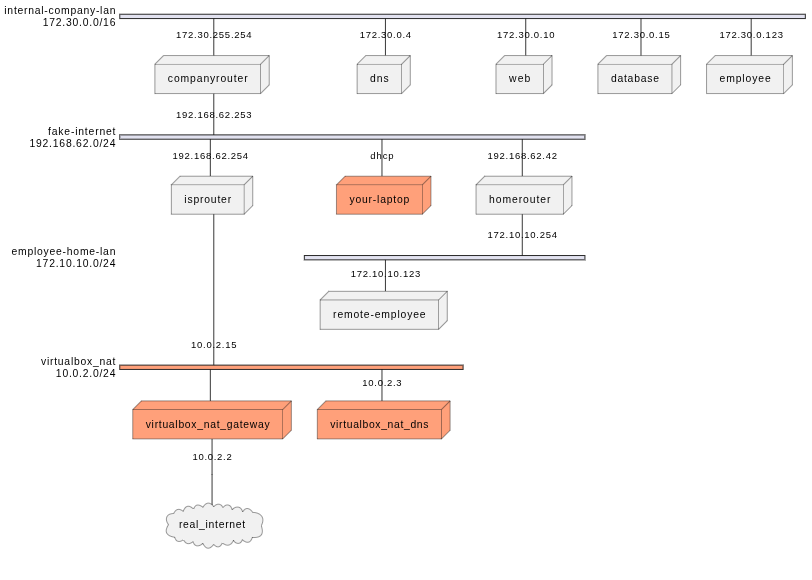
\includegraphics[width=\textwidth]{../graphics/nwdiag_cybersec_adv_env.png}
\caption[Netwerkdiagram testcase 1 in afbeeldingsformaat (PlantUML)]{Afbeeldingsformaat van het netwerkdiagram voor testcase 1 (\emph{Cybersecurity Advanced}), gegenereerd door PlantUML.}
\label{fig:nwdiag_cybersec_adv}
\end{figure}

\subsection{Gegenereerde bestanden}%
\label{subsec:testcase1_gegenereerd}

De converter genereert het ``\texttt{vagrant-hosts.yml}''-bestand in de uitvoermap. Dit bestand bevat voor elke beheerde host een entry met overeenkomend(e) IP-adres(sen) en werkgeheugen, afkomstig uit de ``\texttt{address}''- en ``\texttt{memory}''-attributen in het netwerkdiagram. De routers ``\texttt{companyrouter}'' en ``\texttt{homerouter}'' beschikken elk over meerdere netwerkinterfaces (één per verbonden subnet), wat resulteert in meerdere IP-adresregels per entry.

\begin{codeblock}
\inputminted{yaml}{../plantuml/output/cybersec_adv_env/vagrant-hosts.yml}
\caption[Gegenereerde ``\texttt{vagrant-hosts.yml''} voor testcase 1]{De door de converter gegenereerde \texttt{vagrant-hosts.yml} voor testcase 1 (\emph{Cybersecurity Advanced}).}
\label{code:vagrant_hosts_cybersec}
\end{codeblock}

\subsection{Gekopieerde assets}%
\label{subsec:testcase1_assets}

Naast het gegenereerde ``\texttt{vagrant-hosts.yml}''-bestand kopieert de converter ook een vooraf opgestelde ``\texttt{Vagrantfile}'' naar de uitvoermap. Deze leest de ``\texttt{vagrant-hosts.yml}'' in en voorziet voor elke entry de correcte Vagrant-VM-configuratie, inclusief de VirtualBox-netwerkinstellingen.

\subsection{Beoordeling}%
\label{subsec:testcase1_beoordeling}

Alle beheerde hosts uit de originele labo-omgeving zijn aanwezig in de gegenereerde ``\texttt{vagrant-hosts.yml}''. De ``\texttt{address}''- en ``\texttt{memory}''-attributen uit het netwerkdiagram zijn correct overgenomen en omgezet tot de juiste waarden.
De Vagrant-omgeving kan worden opgestart met het ``\texttt{vagrant up}''-commando zonder verdere manuele aanpassingen.

Ter verduidelijking; de Vagrant-VM's worden hier wel aangemaakt, maar zonder enige Ansible-configuratie. De gegenereerde omgeving is bijgevolg niet functioneel equivalent aan de volledige originele labo-opzet: de subnetten zijn niet onderling verbonden via de routers (``\texttt{companyrouter}'', ``\texttt{isprouter}'', ``\texttt{homerouter}''), de firewall- en NAT-regels ontbreken, en er wordt geen software op onder andere de webserver en databank geïnstalleerd. Deze output kan wel als vertrekpunt gebruikt worden om manuele of aanvullende configuratie (al dan niet via Ansible) nadien toe te passen.

\section{Testcase 2: Full mode (Infrastructure Automation, labo 2)}%
\label{sec:testcase2}

Het tweede labo van het OLOD \emph{Infrastructure Automation} beschrijft het opzetten van een enkel lokaal netwerk (``\texttt{infra.lan}'', ``\texttt{172.16.0.0/16}'') met de volgende hosts:

\begin{itemize}
    \item een primaire DNS-server (``\texttt{srv001}'')
    \item een secundaire DNS-server (``\texttt{srv002}'')
    \item een DHCP-server (``\texttt{srv003}'')
    \item een webserver (``\texttt{srv100}'')
\end{itemize}

De router ``\texttt{r001}'', gebruikerslaptop ``\texttt{your-laptop}'' en het werkstation ``\texttt{ws0001}'' worden niet door de converter beheerd. Deze omgeving wordt opgezet via het \nameref{subsec:fullmode}-gebruiksscenario van de converter.

\subsection{Invoer: netwerk- en implementatiediagram}%
\label{subsec:testcase2_invoer}

Het opgestelde netwerkdiagram (``\texttt{nwdiag\_infra\_auto\_lab\_2\_env.puml}'') bevat één beheerd subnet (``\texttt{infra.lan}''). De niet-beheerde hosts (``\texttt{r001}'', ``\texttt{your-laptop}'' en ``\texttt{ws0001}'') en het volledige ``\texttt{virtualbox\_nat}''-netwerk worden als niet-beheerd gemarkeerd.

\begin{codeblock}
\lstinputlisting[language=plantuml]{../plantuml/input/infra_auto_lab_2_env/nwdiag_infra_auto_lab_2_env.puml}
\caption[Netwerkdiagram testcase 2 in tekstformaat (PlantUML)]{Tekstformaat (``\texttt{nwdiag\_infra\_auto\_lab\_2\_env.puml}'') van het netwerkdiagram voor testcase 2 (\emph{Infrastructure Automation}, labo 2).}
\label{code:nwdiag_infra_auto_lab2}
\end{codeblock}

\begin{figure}[H]
\centering
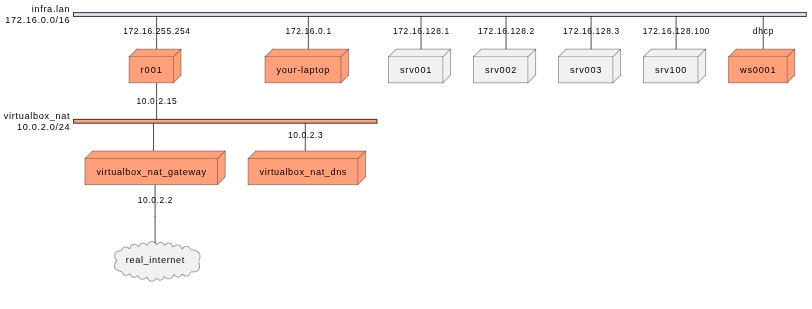
\includegraphics[width=\textwidth]{../graphics/nwdiag_infra_auto_lab_2_env.png}
\caption[Netwerkdiagram testcase 2 in afbeeldingsformaat (PlantUML)]{Afbeeldingsformaat van het netwerkdiagram voor testcase 2 (\emph{Infrastructure Automation}, labo 2), gegenereerd door PlantUML.}
\label{fig:nwdiag_infra_auto_lab2}
\end{figure}

Het opgestelde implementatiediagram (``\texttt{uml\_infra\_auto\_lab\_2\_env.puml}'') stelt ``\texttt{node}''-definites op voor de vier beheerde hosts. De pijlverbindingen vanuit alle ``\texttt{dns\_client}''-componenten naar ``\texttt{srv001.dns\_server\_primary}'' en ``\texttt{srv002.dns\_server\_secondary}'' worden door de converter gebruikt om de DNS-serverconfiguratie en de DHCP-subnettendefinitie correct in te vullen.

\begin{codeblock}
\lstinputlisting[language=plantuml]{../plantuml/input/infra_auto_lab_2_env/uml_infra_auto_lab_2_env.puml}
\caption[Implementatiediagram testcase 2 in tekstformaat (PlantUML)]{Tekstformaat (``\texttt{uml\_infra\_auto\_lab\_2\_env.puml}'') van het implementatiediagram voor testcase 2 (\emph{Infrastructure Automation}, labo 2).}
\label{code:uml_infra_auto_lab2}
\end{codeblock}

\begin{figure}[H]
\centering
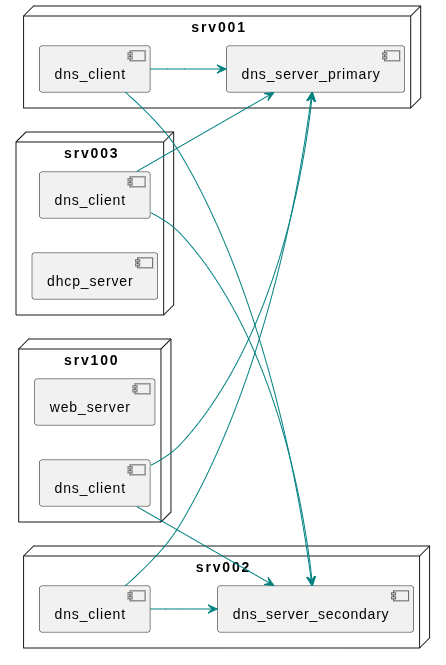
\includegraphics[width=.55\textwidth]{../graphics/uml_infra_auto_lab_2_env.png}
\caption[Implementatiediagram testcase 2 in afbeeldingsformaat (PlantUML)]{Afbeeldingsformaat van het implementatiediagram voor testcase 2 (\emph{Infrastructure Automation}, labo 2), gegenereerd door PlantUML.}
\label{fig:uml_infra_auto_lab2}
\end{figure}

\subsection{Gegenereerde bestanden}%
\label{subsec:testcase2_gegenereerd}

De converter genereert de volgende bestanden in de uitvoermap:

\begin{itemize}
    \item ``\texttt{vagrant-hosts.yml}'': de Vagrant-VM-definities
    \item ``\texttt{ansible/inventory.yml}'': de Ansible inventory
    \item ``\texttt{ansible/site.yml}'': de (hoofd-)playbook
    \item ``\texttt{ansible/host\_vars/srv001.yml}'': de hostvariabelen voor ``\texttt{srv001}''
    \item ``\texttt{ansible/host\_vars/srv002.yml}'': de hostvariabelen voor ``\texttt{srv002}''
    \item ``\texttt{ansible/host\_vars/srv003.yml}'': de hostvariabelen voor ``\texttt{srv003}''
    \item ``\texttt{ansible/host\_vars/srv100.yml}'': de hostvariabelen voor ``\texttt{srv100}''
    \item ``\texttt{ansible/requirements.yml}'': de ``\emph{Ansible Galaxy}''-afhankelijkheden
\end{itemize}

De playbook (``\texttt{site.yml}'') bevat plays in de volgorde bepaald door het topologisch sorteeralgoritme (zie \nameref{subsec:dynamische_bestanden}): hosts met ``\texttt{dns\_server\_primary}'' of ``\texttt{dns\_server\_secondary}'' worden vóór hosts met ``\texttt{dns\_client}'' geconfigureerd, overeenkomstig de ``\texttt{depends\_on}''-relaties in ``\texttt{role-config.yml}''.

\begin{codeblock}
\inputminted{yaml}{../plantuml/output/infra_auto_lab_2_env/ansible/site.yml}
\caption[Gegenereerde ``\texttt{site.yml}'' voor testcase 2]{De door de converter gegenereerde ``\texttt{site.yml}'' voor testcase 2 (\emph{Infrastructure Automation}, labo 2).}
\label{code:site_infra_auto_lab2}
\end{codeblock}

\subsection{Gekopieerde assets}%
\label{subsec:testcase2_assets}

Naast de gegenereerde bestanden kopieert de converter de volgende assets naar de uitvoermap:

\begin{itemize}
\item ``\texttt{Vagrantfile}'': het standaard Vagrant-sjabloon
\item ``\texttt{scripts/}'': de Vagrant-provisioneringsscripts
\item ``\texttt{ansible/roles/web\_server}'': de voorgedefinieerde ``\texttt{web\_server}''-rol
\item ``\texttt{ansible/roles/dns\_server}'': de voorgedefinieerde ``\texttt{dns\_server}''-rol (wordt voor zowel voor ``\texttt{dns\_server\_primary}'' als ``\texttt{dns\_server\_secondary}'' gebruikt)
\item ``\texttt{ansible/roles/dns\_client}'': de voorgedefinieerde ``\texttt{dns\_client}''-rol
\item ``\texttt{ansible/files/ca.crt}'', ``\texttt{ansible/files/ca.key}'', \\``\texttt{ansible/files/db.sql}'', ``\texttt{ansible/files/test.php}'': de statische bestanden benodigd voor de ``\texttt{web\_server}''-rol
\end{itemize}

\subsection{Beoordeling}%
\label{subsec:testcase2_beoordeling}

Alle vier beheerde hosts zijn aanwezig in de gegenereerde uitvoer. De DNS-zone-informatie, de DHCP-subnettendefinitie en de firewall-poortenlijsten zijn correct afgeleid uit de diagraminformatie en het ``\texttt{role-config.yml}''-bestand.

De router ``\texttt{r001}'' is de voornaamste beperking van deze testcase: het doel van deze host wordt door de converter niet ondersteund en is bijgevolg afwezig in de geproduceerde uitvoer. De beheerde hosts beschikken wel over internettoegang via hun eigen VirtualBox NAT-interface, maar onderlinge routering is dus niet geconfigureerd. DNS-queries tussen de hosts onderling blijven wel functioneel, aangezien deze via de gegenereerde DNS-serverconfiguratie verlopen.

\section{Testcase 3: Full mode (Infrastructure Automation, labo 3)}%
\label{sec:testcase3}

Labo 3 van \emph{Infrastructure Automation} bouwt verder op de omgeving van labo 2 door een monitoring-server (``\texttt{srv004}'') toe te voegen. Op deze host wordt Prometheus en Grafana geïnstalleerd via de ``\texttt{monitoring\_server}''-rol. Op alle hosts worden daarnaast ook dienst-specifieke exporters voorzien.

\subsection{Invoer: netwerk- en implementatiediagram}%
\label{subsec:testcase3_invoer}

Het netwerkdiagram (``\texttt{nwdiag\_infra\_auto\_lab\_3\_env.puml}'') is een uitbreiding van het opgestelde netwerkdiagram uit testcase 2 met de toevoeging van de host ``\texttt{srv004}'' (met 2 CPU cores en 2048 MB werkgeheugen).

\begin{codeblock}
\lstinputlisting[language=plantuml]{../plantuml/input/infra_auto_lab_3_env/nwdiag_infra_auto_lab_3_env.puml}
\caption[Netwerkdiagram testcase 3 in tekstformaat (PlantUML)]{Tekstformaat (``\texttt{nwdiag\_infra\_auto\_lab\_3\_env.puml}'') van het netwerkdiagram voor testcase 3 (\emph{Infrastructure Automation}, labo 3).}
\label{code:nwdiag_infra_auto_lab3}
\end{codeblock}

\begin{figure}[H]
\centering
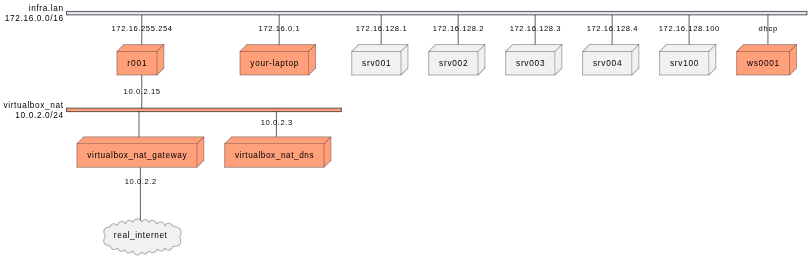
\includegraphics[width=\textwidth]{../graphics/nwdiag_infra_auto_lab_3_env.png}
\caption[Netwerkdiagram testcase 3 in afbeeldingsformaat (PlantUML)]{Afbeeldingsformaat van het netwerkdiagram voor testcase 3 (\emph{Infrastructure Automation}, labo 3), gegenereerd door PlantUML.}
\label{fig:nwdiag_infra_auto_lab3}
\end{figure}

Het implementatiediagram (``\texttt{uml\_infra\_auto\_lab\_3\_env.puml}'') breidt het opgestelde implementatiediagram uit testcase 2 uit door de host/``\texttt{node}'' ``\texttt{srv004}'' toe te voegen, alsook dienst-specifieke exporterrollen voor elke ``\texttt{node}'':

\begin{itemize}
    \item ``\texttt{apache\_exporter}'' voor ``\texttt{srv100}''
    \item ``\texttt{bind\_exporter}'' voor ``\texttt{srv001}'' en ``\texttt{srv002}''
    \item ``\texttt{mysqld\_exporter}'' voor ``\texttt{srv100}''
    \item ``\texttt{node\_exporter}'' voor elke ``\texttt{node}'', inclusief ``\texttt{srv004}''
\end{itemize}

De pijlverbindingen vanuit ``\texttt{srv004.monitoring\_server}'' naar alle exporterrollen worden door de converter gebruikt om de Prometheus scrape targets automatisch op te bouwen (via de ``\texttt{prometheus\_scrape\_configs}''-variabele).

\begin{codeblock}
\lstinputlisting[language=plantuml]{../plantuml/input/infra_auto_lab_3_env/uml_infra_auto_lab_3_env.puml}
\caption[Implementatiediagram testcase 3 in tekstformaat (PlantUML)]{Tekstformaat (``\texttt{uml\_infra\_auto\_lab\_3\_env.puml}'') van het implementatiediagram voor testcase 3 (\emph{Infrastructure Automation}, labo 3).}
\label{code:uml_infra_auto_lab3}
\end{codeblock}

\begin{figure}[H]
\centering
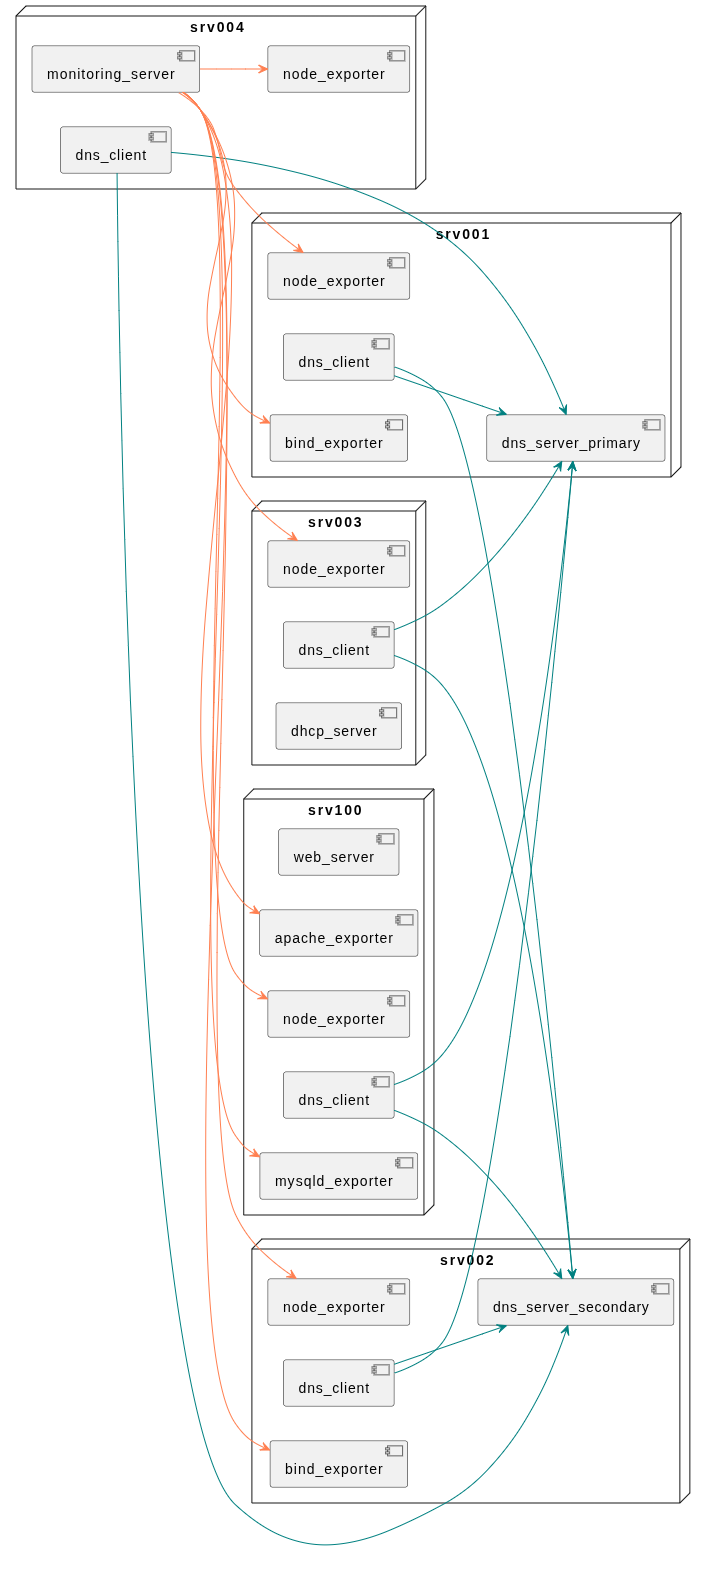
\includegraphics[width=.65\textwidth]{../graphics/uml_infra_auto_lab_3_env.png}
\caption[Implementatiediagram testcase 3 in afbeeldingsformaat (PlantUML)]{Afbeeldingsformaat van het implementatiediagram voor testcase 3 (\emph{Infrastructure Automation}, labo 3), gegenereerd door PlantUML.}
\label{fig:uml_infra_auto_lab3}
\end{figure}

\subsection{Gegenereerde bestanden}%
\label{subsec:testcase3_gegenereerd}

Ten opzichte van testcase 2 zijn de volgende (extra) bestanden gegenereerd/uitgebreid:

\begin{itemize}
    \item ``\texttt{ansible/host\_vars/srv004.yml}'': de hostvariabelen voor ``\texttt{srv004}''
    \item Een uitgebreide ``\texttt{ansible/requirements.yml}'' met de \\``\texttt{prometheus.prometheus}''- en ``\texttt{grafana.grafana}''-``\emph{Ansible Galaxy}''-collecties
    \item De hostvariabelen van ``\texttt{srv001}'' en ``\texttt{srv002}'' zijn uitgebreid voor \\``\texttt{bind\_exporter}''
    \item De hostvariabelen van ``\texttt{srv100}'' zijn uitgebreid voor ``\texttt{apache\_exporter}'' en ``\texttt{mysqld\_exporter}''
\end{itemize}

De hostvariabelen van \texttt{srv004} bevatten de automatisch gegenereerde \\``\texttt{prometheus\_scrape\_configs}''-waarde, opgebouwd op basis van alle exporterverbindingen in het implementatiediagram.

\begin{codeblock}
\inputminted{yaml}{../plantuml/output/infra_auto_lab_3_env/ansible/host_vars/srv004.yml}
\caption[Gegenereerde \texttt{host\_vars/srv004.yml} voor testcase 3]{De door de converter gegenereerde hostvariabelen voor \texttt{srv004}. De \texttt{prometheus\_scrape\_configs}-waarde is automatisch samengesteld op basis van de pijlverbindingen in het implementatiediagram.}
\label{code:hostvars_srv004}
\end{codeblock}

\subsection{Gekopieerde assets}%
\label{subsec:testcase3_assets}

Ten opzichte van testcase 2 worden de volgende extra assets gekopieerd:
\begin{itemize}
    \item ``\texttt{ansible/roles/monitoring\_server}'': \\de voorgedefinieerde ``\texttt{monitoring\_server}''-rol
    \item ``\texttt{ansible/files/grafana/default.yml}'': \\het configuratiebestand voor Grafana
    \item ``\texttt{ansible/files/grafana/dashboards/apache\_exporter.json}'': \\het Grafana-dashboard voor ``\texttt{apache\_exporter}''
    \item ``\texttt{ansible/files/grafana/dashboards/bind\_exporter.json}'': \\het Grafana-dashboard voor ``\texttt{bind\_exporter}''
    \item ``\texttt{ansible/files/grafana/dashboards/mysqld\_exporter.json}'': \\het Grafana-dashboard voor ``\texttt{mysqld\_exporter}''
    \item ``\texttt{ansible/files/grafana/dashboards/node\_exporter.json}'': \\het Grafana-dashboard voor ``\texttt{node\_exporter}''
\end{itemize}

\subsection{Beoordeling}%
\label{subsec:testcase3_beoordeling}

De uitvoer voor labo 3 is functioneel equivalent aan de manueel opgestelde Ansible-configuratie uit de originele labo-omgeving. Alle vijf beheerde hosts zijn aanwezig, de exporterconfiguraties zijn correct gegenereerd en de Prometheus scrape-configuratie reflecteert nauwkeurig de verbindingen uit het implementatiediagram.

De beperking met betrekking tot ``\texttt{r001}'' geldt ook hier; zie \nameref{subsec:testcase2_beoordeling}. Daarnaast veronderstelt de gegenereerde ``\texttt{monitoring\_server}''-configuratie dat de DNS-servers reeds operationeel zijn vóór de Prometheus-installatie; dit is gegarandeerd door de ``\texttt{depends\_on}''-relaties in ``\texttt{role-config.yml}'' en straalt zich uit in de resulterende volgorde in ``\texttt{site.yml}''.

%%=============================================================================
%% Conclusie
%%=============================================================================

\chapter{Conclusie \& Discussie}%
\label{ch:conclusie_discussie}

% TODO: Trek een duidelijke conclusie, in de vorm van een antwoord op de
% onderzoeksvra(a)g(en). Wat was jouw bijdrage aan het onderzoeksdomein en
% hoe biedt dit meerwaarde aan het vakgebied/doelgroep? 
% Reflecteer kritisch over het resultaat. In Engelse teksten wordt deze sectie
% ``Discussion'' genoemd. Had je deze uitkomst verwacht? Zijn er zaken die nog
% niet duidelijk zijn?
% Heeft het onderzoek geleid tot nieuwe vragen die uitnodigen tot verder 
%onderzoek?

% \lipsum[76-80]

\section{Conclusie}%
\label{sec:conclusie}

Om op de centrale onderzoeksvraag van deze bachelorproef te antwoorden, is een proof-of-concept converter ontwikkeld genaamd PlantUML2Ansible, die netwerk- en implementatiediagrammen, geschreven in PlantUML-code, als invoer aanneemt en een volledig IaC- en `\emph{configuration management}'-ondersteunde omgeving (aangeboden door Vagrant en Ansible, respectievelijk) als uitvoer produceert.

Naast dit primaire gebruiksscenario (\nameref{subsec:fullmode}) is er ook een alternatief scenario ontwikkeld om enkel een Vagrant-omgeving te produceren (\nameref{subsec:iaconlymode}).

Bestaande labo-omgevingen uit bepaalde OLODS binnen de opleiding \emph{Toegepaste Informatica} (\emph{Cybersecurity Advanced} en \emph{Infrastructure Automation}) zijn herwerkt als bruikbare invoer voor de converter (zijnde netwerk- en/of implementatiediagrammen) en zijn, binnen de beperkingen van het script, met succes omgezet naar functionele omgevingen.
De initiële labo-omgeving van \emph{Cybersecurity Advanced} is via de ``IaC-only mode'' volledig gereproduceerd kunnen worden als  een Vagrant-ondersteunde omgeving.
De labo's 2 en 3 uit \emph{Infrastructure Automation} zijn ook via de ``full mode'' gerecreëerd als Vagrant- en Ansible-ondersteunde omgeving, maar zonder de router \texttt{r001}.

Deze resultaten tonen dus aan dat het technisch haalbaar is om, op basis van PlantUML-bronbestanden, volledige en functionele omgevingen te genereren -- zonder manuele tussenkomst van de gebruiker.

Tegelijkertijd kent de proof-of-concept een aantal beperkingen die de scope van het huidige onderzoek afbakenen. De ``full mode'' ondersteunt slechts één netwerk, het ondersteunde gastbesturingssysteem wordt beperkt tot \emph{AlmaLinux} 9, en de invoerdiagrammen moeten voldoen aan een welomschreven en beperkt subset van de PlantUML-syntax.

De meerwaarde van deze oplossing situeert zich voornamelijk in de educatieve context waarvoor ze ontworpen is. Docenten binnen de opleiding \emph{Toegepaste Informatica} op HOGENT kunnen met deze tool sneller nieuwe labo-omgevingen ontwerpen en deze tegelijk voorzien van functionele code om deze effectief op te zetten en te configureren. De kloof tussen de ontwerpfase (UML-diagram) en de implementatiefase (uitgerolde omgeving) wordt zo met andere woorden aanzienlijk verkleind.

Voor studenten kan de tool de link tussen deze twee fases juist alsmaar meer verduidelijken, en de drempel verlagen om nieuwe infrastructuur-gerelateerde ideeën al experimenterend vorm te geven.

\section{Discussie}%
\label{sec:discussie}

De beperkingen van deze proof-of-concept leggen verschillende fundamenten waarop toekomstige uitbreidingen verder gebouwd kunnen worden.

Het ondersteunen voor meerdere netwerken in beide modi is technisch mogelijk, mits de configuratie van routering (en de gerelateerde firewallregels) wordt verwerkt in de logica van het script. Daarnaast moet er, onder andere, een uitbreiding van de DNS-zone-generatielogica uitgevoerd worden, alsook een herziene aanpak voor de toewijzing (van het IP-adres) van de Ansible \texttt{control}-node.

De beperking van \emph{AlmaLinux} 9 als gastbesturingssysteem kan geremedieerd worden door de configuratie van de rollen niet meer afhankelijk te maken van de bestaande rollen die gebruikt worden binnen de opleiding \emph{Toegepaste Informatica}. Door over te stappen naar meer distributie-agnostische modules in deze  nieuwe rollen, zou de converter ook andere distributies kunnen ondersteunen, waaronder de nieuwere \emph{AlmaLinux} 10 en misschien zelfs Ubuntu Server of Alpine Linux.

Het huidige \texttt{role-config.yml}-bestand bevat momenteel slechts een beperkt aantal voorgedefinieerde rollen. Hoewel het bestand alvast een modulaire basis heeft, is het op dit moment niet mogelijk om nieuwe rollen (zelfs met de minste complexiteit) te definiëren zonder de broncode van het script te wijzigen.

Andere, minder cruciale uitbreidingen zouden de volgende kunnen inhouden:
\begin{itemize}
    \item Compatibiliteit met IPv6
    \item Ondersteuning voor andere IaC- (Terraform, OpenTofu, \ldots) en `\emph{configuration management}'-backends (Puppet, Chef, \ldots)
    % \item Grafische gebruikersinterface of integraties met IDE's via plugins (bijvoorbeeld een `\emph{Visual Studio Code}'-extensie)
    \item Formele validatie van de PlantUML-invoer en de Vagrant- en Ansible-uitvoer via geïntegreerde linters
\end{itemize}

%---------- Bijlagen -----------------------------------------------------------

\appendix

\chapter{Onderzoeksvoorstel}

Het onderwerp van deze bachelorproef is gebaseerd op een onderzoeksvoorstel dat vooraf werd beoordeeld door de promotor. Dat voorstel is opgenomen in deze bijlage.

%% TODO: 
\section*{Samenvatting}

% Kopieer en plak hier de samenvatting (abstract) van je onderzoeksvoorstel.
Op HOGENT, binnen de opleiding Toegepaste Informatica en meerbepaald het keuzetraject ``System \& Network Administrator'', worden er OLODs (opleidingsonderdelen) gegeven die aan de hand van labo's bijdragen aan het leren beheren van serverinfrastructuren. Deze infrastructuren worden geïmplementeerd aan de hand van netwerk- en implementatiediagrammen, ontworpen met UML-modeling software.
De probleemstelling voor deze bachelorproef vertrekt vanuit het foutgevoelige en tijdrovende proces waarbij (complexe) UML-diagrammen eerst geïnterpreteerd en daarna manueel vertaald worden naar een configureerbare infrastructuur.
De hoofdonderzoeksvraag is hoe men, voor een potentiële serverinfrastructuur, netwerk- en implementatiediagrammen (meerbepaald in tekstuele vorm via PlantUML/MermaidJS) met zo weinig mogelijk manuele interventie kan omzetten naar een overeenkomende, gebruiksklare omgeving ondersteund door ``configuration management''-code (zoals Ansible, Puppet of Chef).
De doelstelling van dit onderzoek is om een proof-of-concept transpiler te ontwikkelen die gegeven netwerk- en implementatiediagrammen als invoer rechtstreeks kan vertalen naar ``configuration management''-code als uitvoer. 
De geplande testomgeving zal bestaan uit 2 tot 3 reeds uitgerolde (virtuele) servers (al dan niet via Infrastructure-as-Code tools), en zullen bestaan uit een web-, DNS- en monitoringserver (zonder nog eventuele uitbreidingen).
Qua methodologie wordt er eerst een studie naar transpilers uitgevoerd, parallel met een evaluatie van te gebruiken tools (PlantUML, MermaidJS, Ansible, Puppet en Chef). Vervolgens wordt de testomgeving ontworpen (via UML-diagrammen), opgezet en gedocumenteert. Dan wordt de transpiler ontwikkeld en ten slotte systematisch getest tegen (onder andere) de kwaliteit en idempotentie van de uitvoer.
Verwacht wordt dat deze oplossing een meerwaarde biedt voor docenten (en studenten): zij zouden hiermee sneller en efficiënter nieuwe labo-omgevingen kunnen ontwerpen en deze tegelijk voorzien van bijkomende ``configuration management''-code, aangezien de kloof tussen de ontwerp- en implementatiefase zo wordt verkleind.

% Verwijzing naar het bestand met de inhoud van het onderzoeksvoorstel
\input{../voorstel/voorstel-inhoud}

%%---------- Andere bijlagen --------------------------------------------------
% TODO: Voeg hier eventuele andere bijlagen toe. Bv. als je deze BP voor de
% tweede keer indient, een overzicht van de verbeteringen t.o.v. het origineel.
%\input{...}

%%---------- Backmatter, referentielijst ---------------------------------------

\backmatter{}

\setlength\bibitemsep{2pt} %% Add Some space between the bibliograpy entries
\printbibliography[heading=bibintoc]

\end{document}
